%!TEX root = ../Allnew-Workspace.tex
\mychapter{지수법칙}{}
\section{중학교 지수법칙 : 자연수 지수}
중학교에서 배운 지수법칙은 엄밀히 따지면 음이 아닌 정수\mn{$0$과 자연수}인 지수에 대해서만 다룹니다. 자연수 $m$, $n$에 대하여 다음과 같은 지수법칙이 성립합니다.

\begin{enumerate}[label=\onum*]
  \item $a^m \times a^n = a^{m+n}$
  \item $a^m \div a^n =
  \begin{cases}
  \:\:a^{m-n}& (m>n)\\
  \:\:\:1&(m=n)\\
  \:\dfrac{1}{a^{n-m}}& (m<n)
  \end{cases}$
  \item $\left( a^m \right)^{n} = a^{mn}$
\end{enumerate}

\section{고등학교 지수법칙 : 표현은 일관적으로, 의미는 더 넓게 확장하기}
고등학교 \cnm{수학 I}에서는 중학교때 배웠던 수 체계의 확장에 따라 지수법칙을 확장해나갈 것입니다. 중학교 지수법칙의 일관성을 지켜나가면서 지수 자리에 들어갈 수를 점점 늘려나가면서 의미를 더 넓히는 것이지요. 차례대로 정수, 유리수, 무리수이고, 유리수와 무리수에 대한 지수법칙이 정의되면 실수 전체에 대한 지수법칙으로 확장한 것이라 말할 수 있을 것입니다.

\subsection{정수 지수 : 역수를 표현하기 위한 지수의 확장}
지수법칙 ②는 $m$과 $n$의 대소관계에 따라 다르게 정의되었습니다. 이를 항상 $a^{m-n}$이 되도록 자연스럽게 정의하면 지수의 범위를 정수로 확장할 수 있습니다.
\begin{enumerate}[label={\onum*}]
    \item $m>n$ \\
    기존과 같이 $a^{m-n}$입니다.
    \item $m=n$\\
    $a^m \div a^n = a^{m-n}=a^0$이므로, 지수가 $0$입니다. 원래의 식을 연산해보면 $a^m \div a^n = a^m \div a^m = 1$입니다. 따라서 정수 $0$에 대하여 $a^0=1$이라 정의할 수 있습니다. 
    \item $m<n$\\
    $a^m \div a^n = a^{m-n}$이므로, 지수가 음의 정수입니다. 원래의 식을 연산해보면 $a^m \div a^n=\dfrac{1}{a^{n-m}}$입니다. 따라서 음의 정수 $m-n$에 대하여 $a^{m-n}=\dfrac{1}{a^{n-m}}$이라 정의할 수 있습니다. 즉 음의 정수를 지수 자리에 놓일 수 있도록 함으로써, 단순히 거듭제곱만 표현할 수 있던 지수의 쓰임새를 넓힌 것입니다. 
\end{enumerate}
이렇게 새로이 정의된 정수 지수 $k \in \mathbb Z$에 대해서도 기존의 지수법칙이 모두 성립합니다. 

\subsection{유리수 지수 : 거듭제곱근을 표현하기 위한 지수의 확장}
%지수법칙 ③을 이용하여 지수의 범위를 유리수로 확장할 수 있습니다. 예시를 통해 생각해봅시다.

우리는 $x^2 = 2$인 양의 실수가 $x=\sqrt{2}$임을 알고 있습니다. 이때 $x=2^r$라 해봅시다. $\left( 2^r \right)^2$에서 지수법칙이 그대로 성립한다면  $\left( 2^r \right)^2=2^{2r}$가 됩니다. 이 값이 $2$와 같은데, $2=2^1$이므로 $2^{2r}= 2^1$입니다. 따라서 $r=\dfrac{1}{2}$입니다.

같은 방법으로 이를 확장하면 $2\expo{\tfrac{1}{m}} = \sqrt[m]{2}$이고, $2\expo{\tfrac{n}{m}} = \sqrt[m]{2^n}$입니다. 따라서 \mbox{거듭제곱근,} 거듭제곱과 거듭제곱근이 섞인 경우 등을 모두 유리수 지수로 표현할 수 있습니다. 즉 유리수를 지수 자리에 놓일 수 있도록 함으로써 지수의 쓰임새를 더욱 넓힌 것입니다. 

\subsection{무리수 지수 : 로그(함수)와 지수함수를 정의하기 위한 지수의 확장}
우리가 지금까지 배운 내용을 토대로 $2^1= 2$, $2^2=4$임을 알지만, $2^x=3$인 $x$의 정체가 무엇인지 알기는커녕, 존재하는지조차 알지 못합니다. 이는 우변이 $3$일때 뿐만 아니라 거듭제곱, 거듭제곱근, 그리고 그들의 역수로 표현될 수 없는 모든 양의 실수 $k$에 대해서 해당되는 이야기입니다. 교과서에서는 이러한 실수 $x$가 임의의 양의 실수 $k$마다 오직 하나 존재함이 \dotemph{알려져 있다}고 합니다.

한편, $2^{\sqrt{2}}$의 정체가 무엇인지 알기는커녕, 정의되는지조차 알지 못합니다. 이는 지수에 무리수가 들어가는 모든 경우에 대해서 마찬가지입니다. 교과서에서는 $2^{\sqrt{2}}$의 값이 한 실수의 값을 가진다는 사실이 \dotemph{알려져 있다}고 합니다.\mn{심지어 교과서는 이를 설명하는 과정에서 아직 배우지도 않은 `함수의 극한'의 개념을 슬쩍 끼워넣는 만행을 저지르기도 합니다.}{} 이는 $2^{\pi}$와 같은 다른 무리수에 대해서도 마찬가지입니다.

이 \dotemph{알려진} 두 가지의 사실을 인정하기로 약속해야 논의를 이어갈 수 있습니다. 전자를 통해 비로소 로그를 정의하고, 뒤에서 곧 배울 로그함수의 정의역이 양수 전체의 집합이고, 치역이 실수 전체의 집합임을 이야기할 수 있습니다. 후자를 통해 비로소 뒤에서 곧 배울 지수함수의 정의역이 실수 전체의 집합이고, 치역이 양수 전체의 집합임을 이야기할 수 있습니다.
\clearpage
\section{로그}
\subsection{로그의 정의}
$a^x = N$이 성립할 때, $x$는\begin{center}
  \textbf{\color{cyan}$a$의 지수 자리에 놓이면 연산 결과를 $N$으로 만들어주는 수}
\end{center}라고 생각할 수 있습니다. 이 의미를 그대로 담아 표현하기 위한 수단이 로그입니다.

예를 들어, 앞서 논의한 바에 따르면 $2^x=3$인 $x$의 값은 분명히 존재하며, 우리는 그 값을 표현할 수 있는 방법이 필요합니다. 따라서 그러한 수를 $\log_2 3$이라 표기하기로 약속하면, 정의에 의해 $2^{\log_2 3} = 3$이 성립합니다.\mn{절대 아래의 공식 ⑤에 의해 자리를 바꿔서 $2^{\log_2 3} = 3^{\log_2 2} = 3$이라고 하면 안 됩니다! 로그의 정의에 의해 곧바로 \mbox{$3$이라고} 해야 합니다.}{}

$1$이 아닌 양수 $a$와 양수 $N$에 대하여 $a^x = N$일 때, $x = \log _a N$이라 표기합니다. 이때 $a$를 이 로그의 밑, $N$을 이 로그의 진수라 합니다.
\subsection{로그의 성질}
로그는 지수에서 파생되었으므로, 지수의 성질과 지수법칙을 이용해 로그의 성질을 끌어낼 수 있습니다.
\begin{enumerate}[label=\onum*]
  \item $a ^{\log_a b} = b$, $\log_a a = 1$, $\log_a 1 = 0$
  \item $\log_a b + \log_a c = \log_a bc$, $\log_a b - \log_a c = \log_a \dfrac{b}{c}$
  \item $\log_{a^p} b^q = \dfrac{q}{p}\log_a b$
  \item $\log_a b = \dfrac{\log_c b}{\log_c a} = \dfrac{1}{\log_b a}$
  \item $a ^{\log_b c} = c^{\log_b a}$
\end{enumerate}



\clearpage


\section{지수함수와 로그함수의 정의}
\subsection{지수함수}
일반적으로 $a$가 $1$이 아닌 양수일 때, 임의의 실수 $x$에 대하여 $a^x$의 값은 하나로 정해집니다. 따라서 $x$에 $a^x$의 값을 대응시키는 함수 $y=a^x$를 생각할 수 있습니다. 이 함수를 `$a$를 밑으로 하는 \term{지수함수}{}'라고 합니다.\mn{앞으로 지수함수를 언급할 때 밑인 $a$는 $1$이 아닌 양수인 것으로 생각하기로 합시다.}{} 지수함수의 정의역은 실수 전체의 집합이고, 치역은 양의 실수 전체의 집합입니다.

\subsection{지수함수 $f$를 원함수로 하는 대거역함수 $x=f^{-1}\left(y\right)$}
지수함수 $f\left( x \right) =a^x$은 실수 전체의 집합에서 양의 실수 전체의 집합으로의 일대일대응이므로 역함수를 갖습니다.\mn{만약 지수함수의 공역이 실수 전체의 집합이라면 일대일대응이 아닌 일대일함수입니다. 본문에서는 지수함수의 공역을 양의 실수 전체의 집합으로 생각한 것입니다.}{} 이제 $f\left( x \right) =a^x $를 원함수로 하는 역함수 $x = f^{-1}(y)$를 구해봅시다. 로그의 정의에 의하여 $y=a^x \Longleftrightarrow x=\log_a y$이므로 $f^{-1}\left( y \right) = \log_a y$입니다. 이때 $x$와 $y$는 원함수에서와 동일하므로 $x$는 모든 실수, $y$는 모든 양수입니다.

\subsection{로그함수 : 지수함수 $f$의 새함역함수 $y=f^{-1}\left(x\right)$}
이제 `새로운 함수로서의 역함수'를 생각하기 위해 $y$와 $x$의 자리를 서로 바꾸면 새로운 함수 $y=\log_a x$를 얻습니다. 이때 이 새로운 함수에서 $x$는 모든 양수, $y$는 모든 실수입니다.  이렇게 얻은 함수 $y=\log_a x$를 `$a$를 밑으로 하는 \term{로그함수}{}'라 합니다.\mn{앞으로 로그함수를 언급할 때 밑인 $a$는 $1$이 아닌 양수인 것으로 생각하기로 합시다.}{} 로그함수의 정의역은 양의 실수 전체의 집합이고, 치역은 실수 전체의 집합입니다.
\clearpage
\section{지수함수와 로그함수의 그래프}

\begin{figure}[h]\centering \subfloat[][]{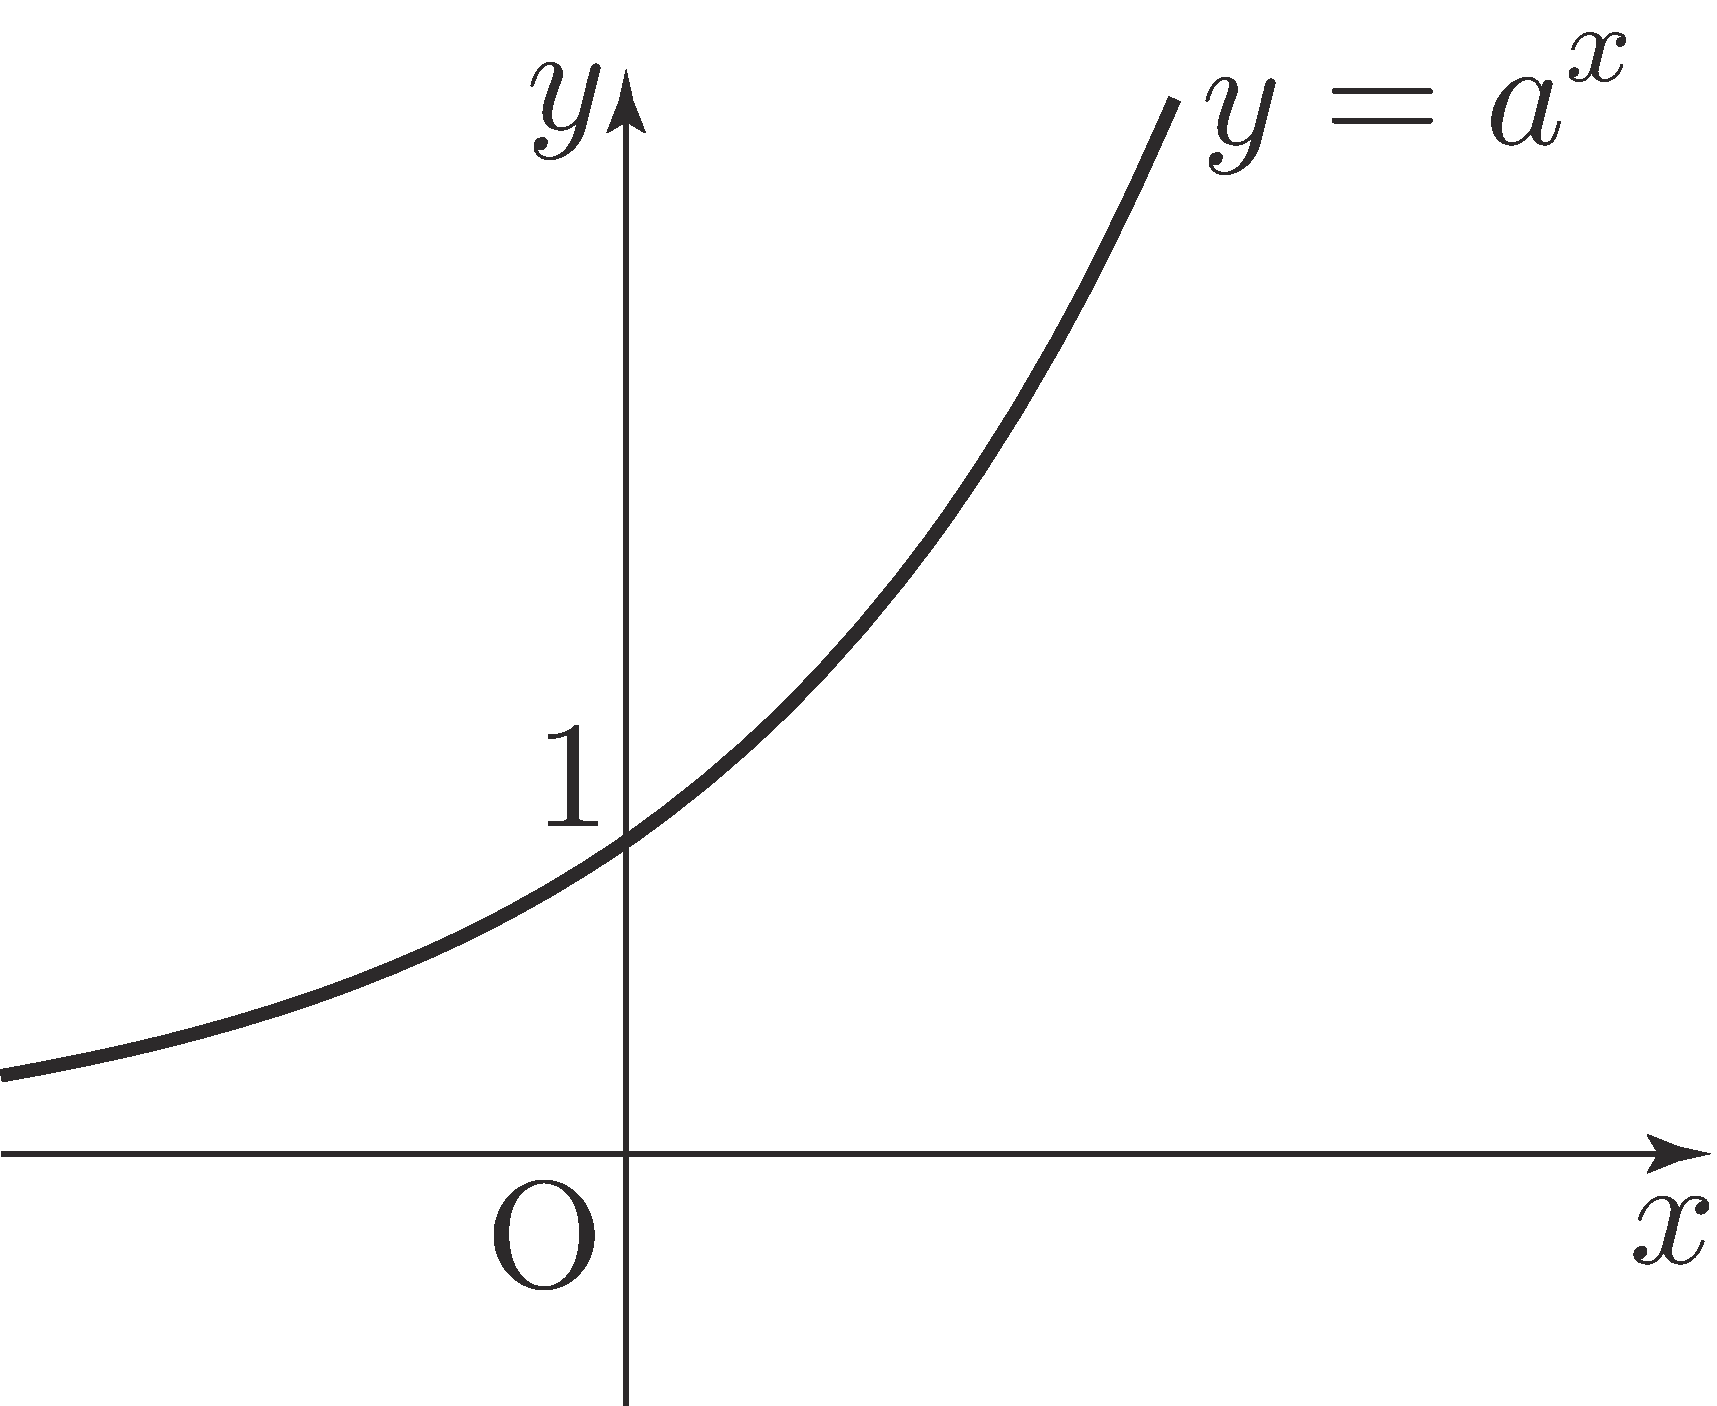
\includegraphics[scale=\pgfkeysvalueof{picsize}]{DBs/pic/zert_01_1.pdf}}\
\qquad\qquad
\centering \subfloat[][]{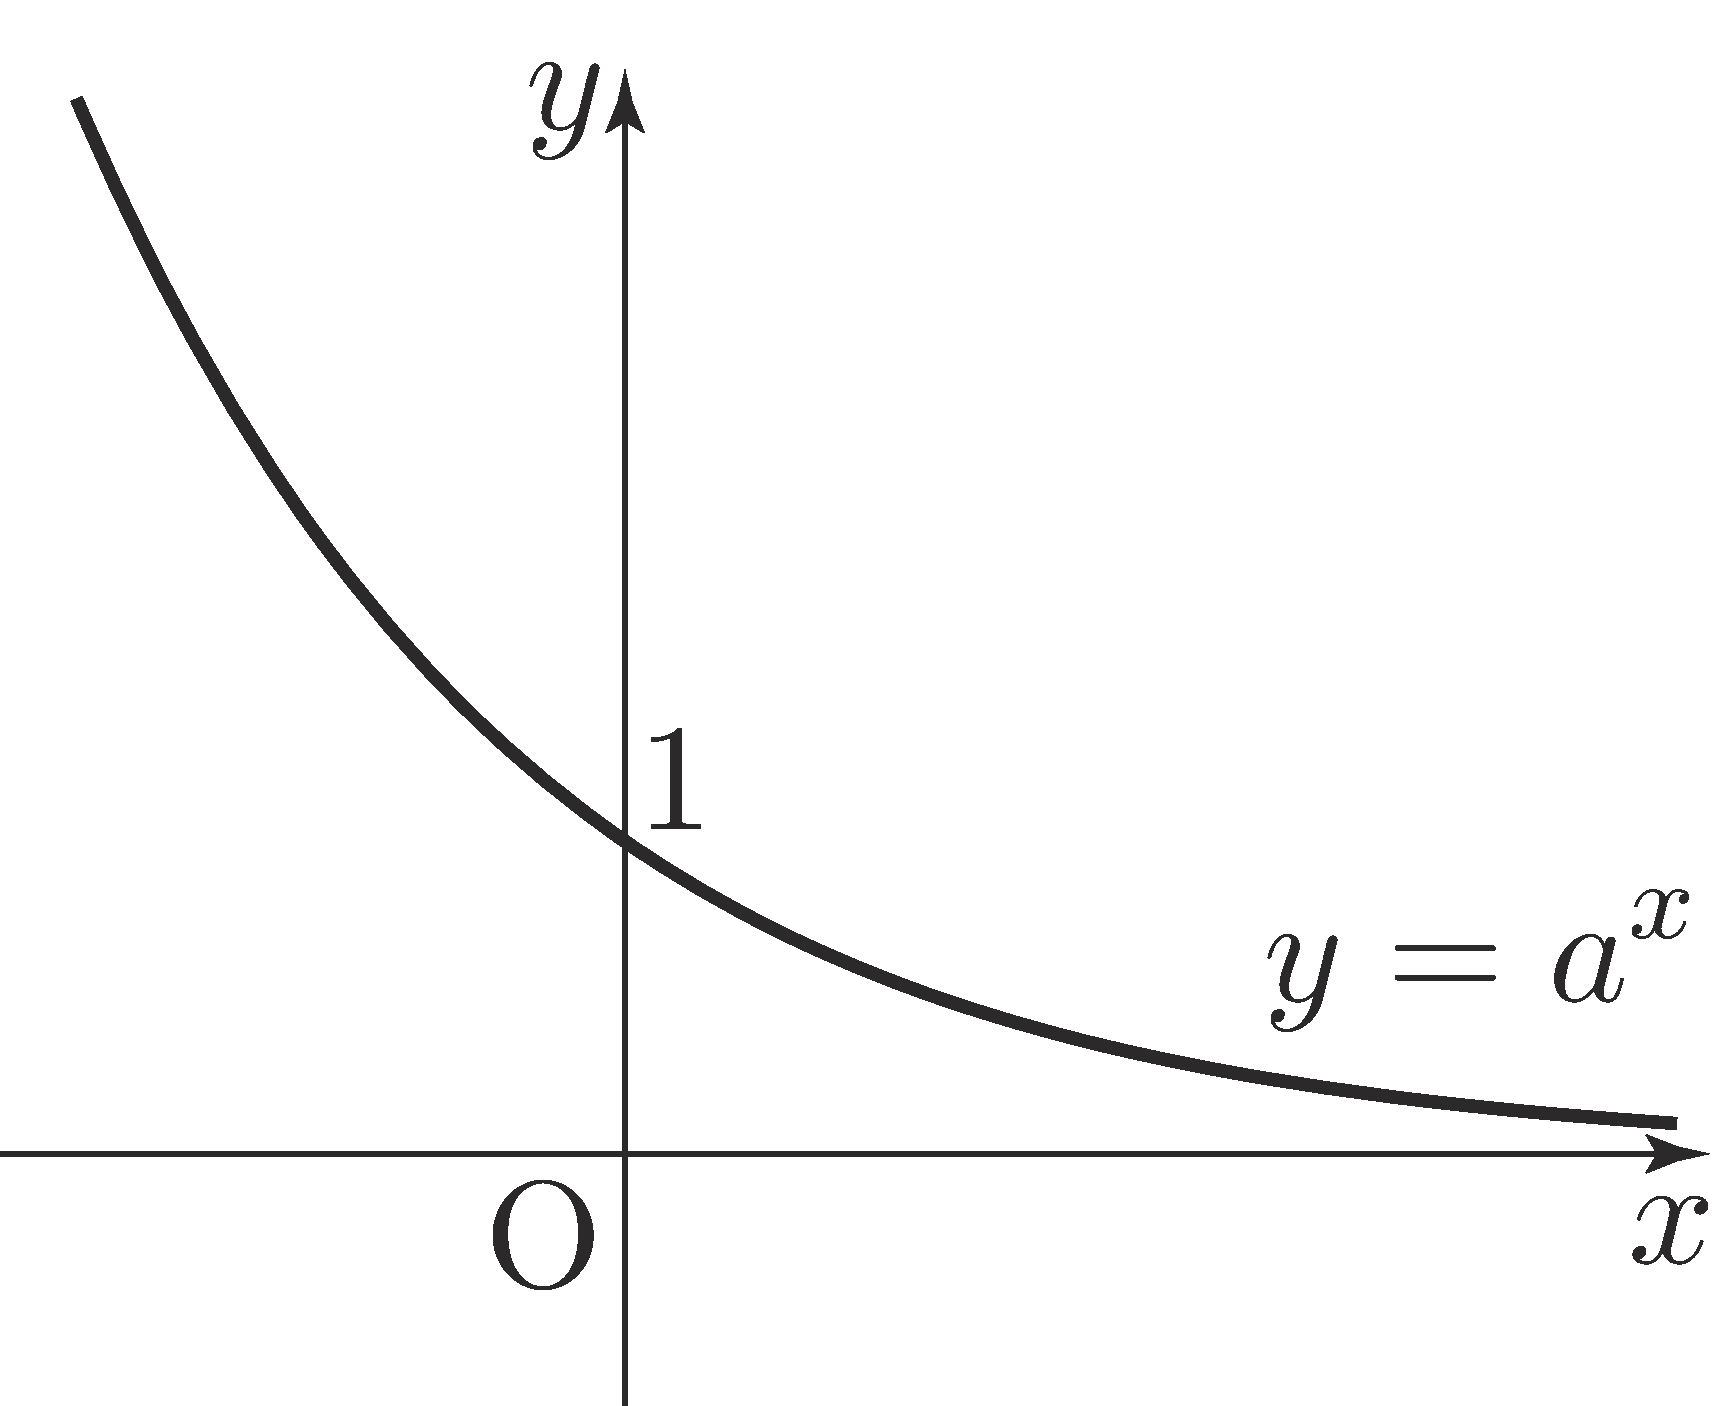
\includegraphics[scale=\pgfkeysvalueof{picsize}]{DBs/pic/zert_01_2.pdf}}\
\end{figure}


지수함수 $y=a^x$에서 $x=0$을 대입하면 $a$의 값에 관계 없이 $y=1$이므로, 지수함수의 그래프는 $a$의 값에 관계 없이 $\xy{0}{1}$을 지납니다. $a>1$이면 (a)와 같고, $0<a<1$이면 (b)와 같습니다.

\begin{figure}[h]
	\centering \subfloat[][]{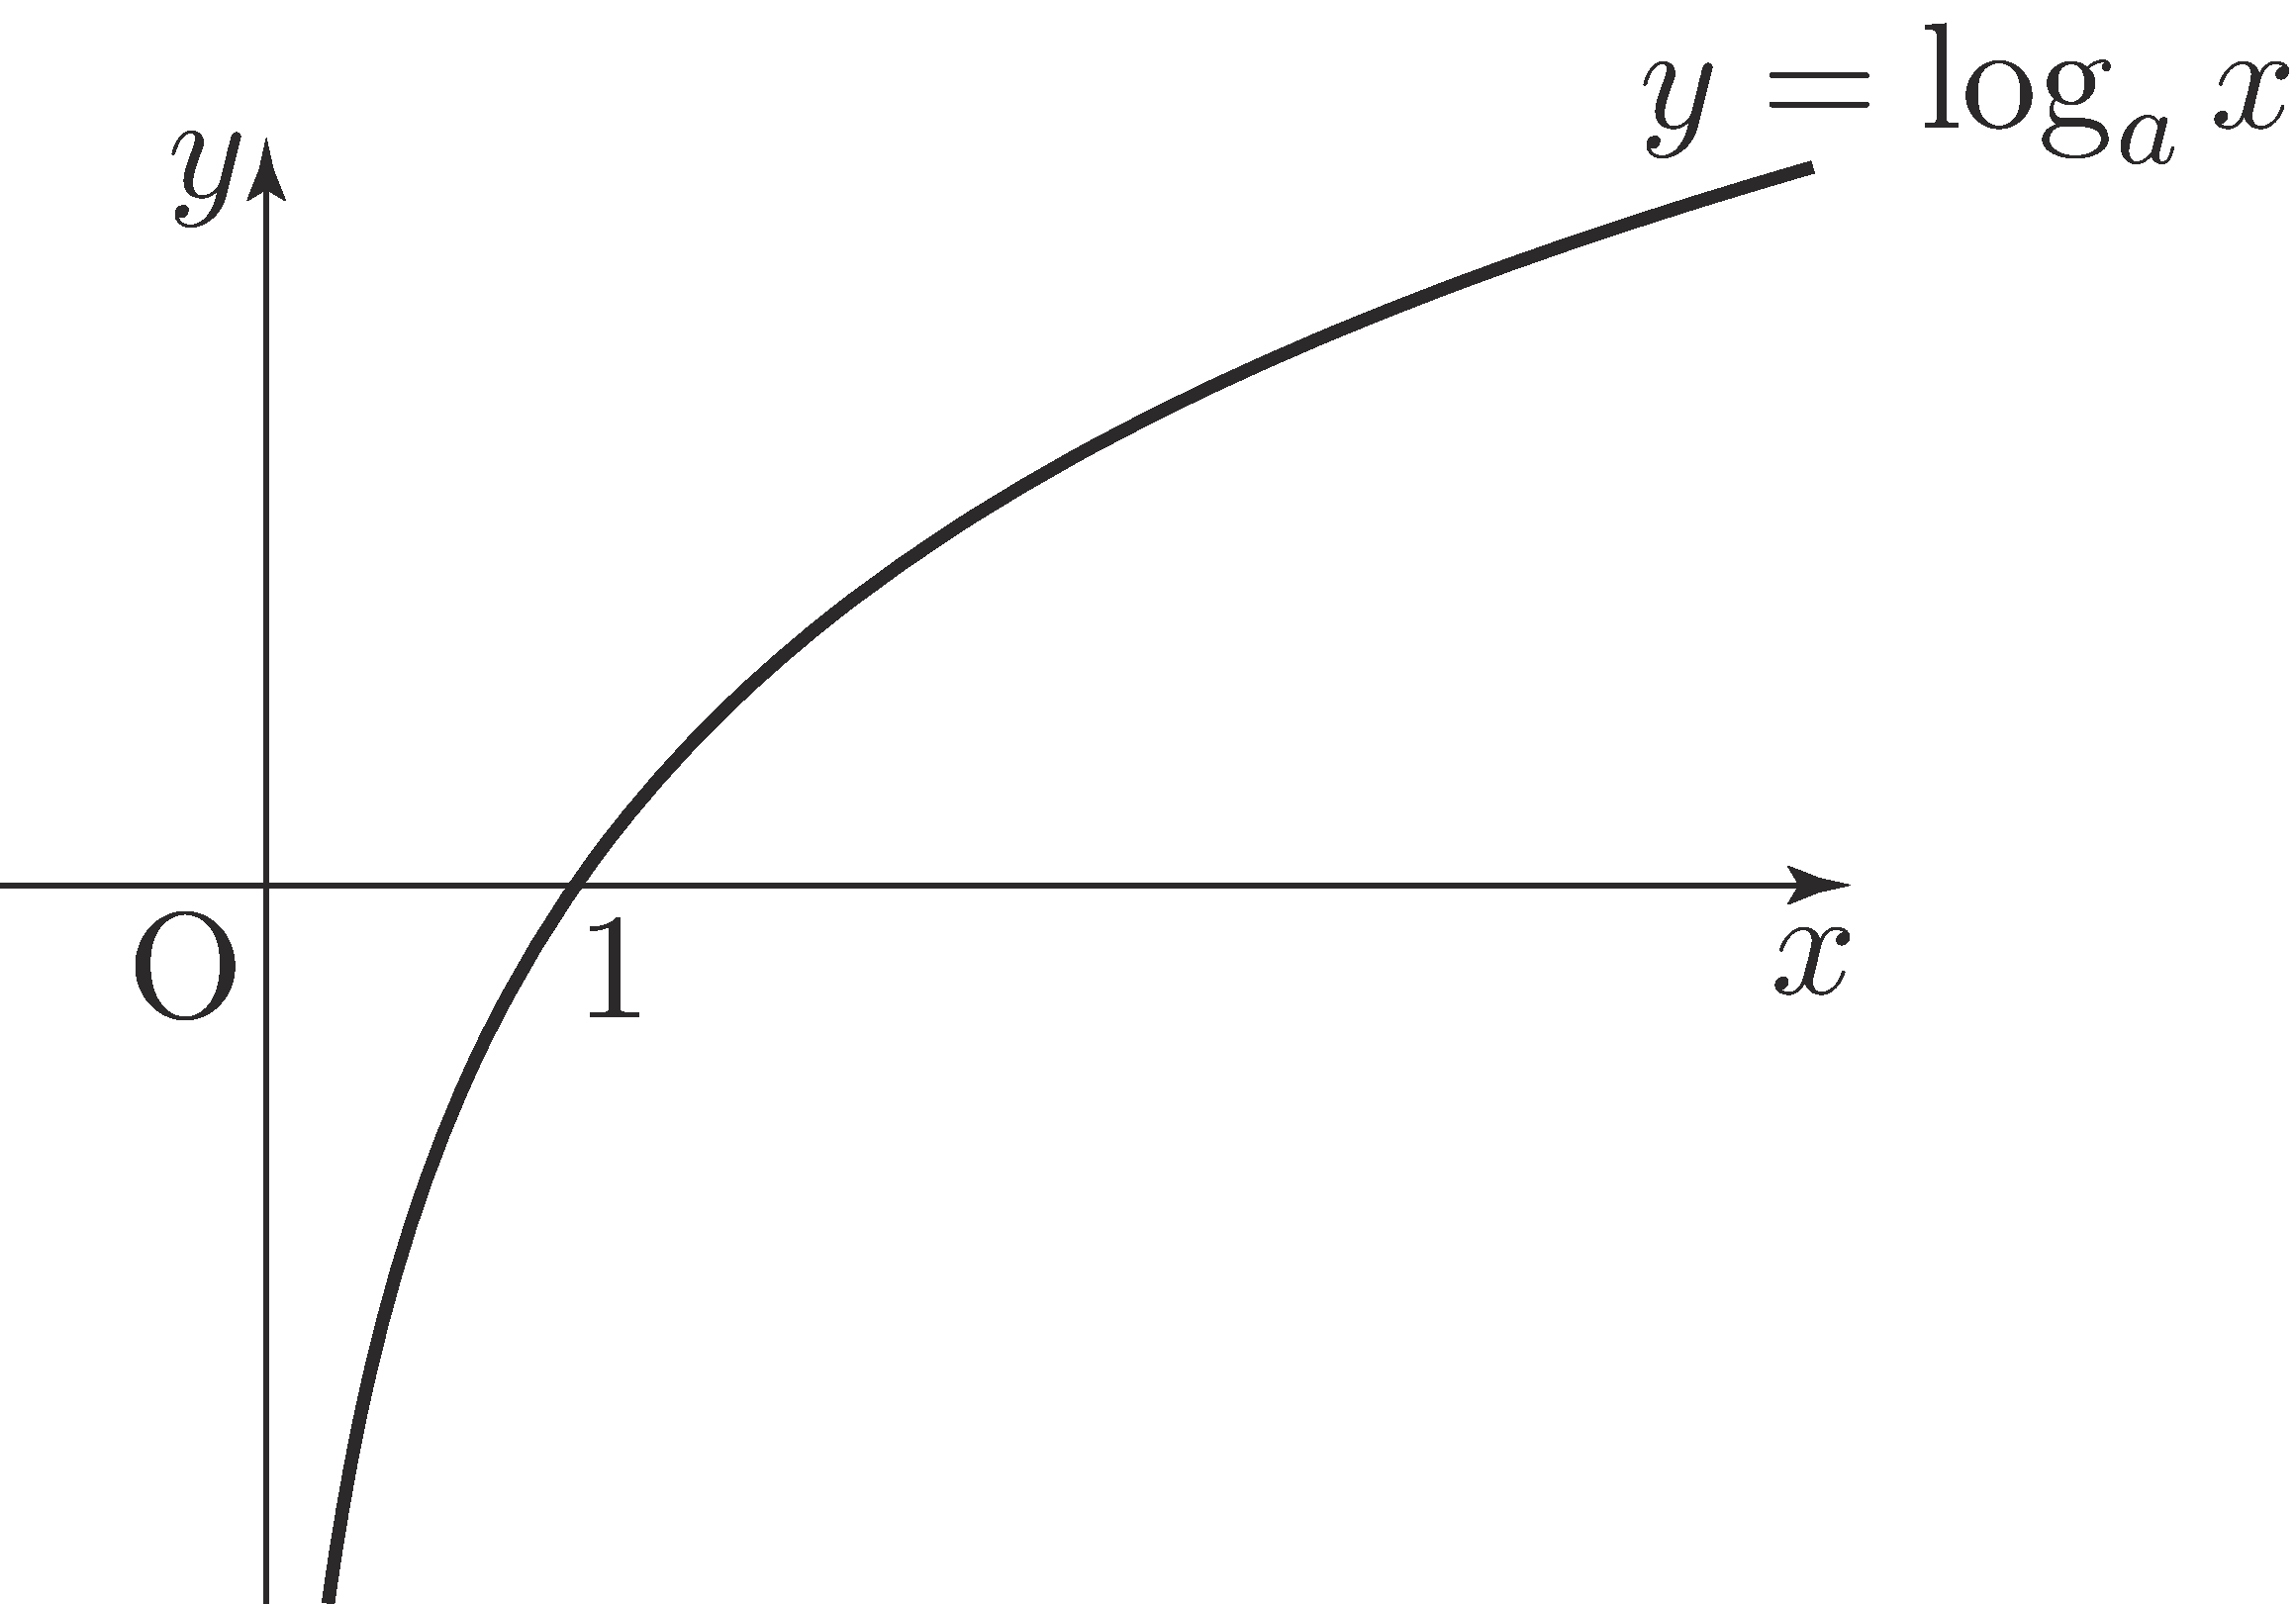
\includegraphics[scale=\pgfkeysvalueof{picsize}]{DBs/pic/zert_02_1.pdf}}\
	\qquad\qquad
	\centering \subfloat[][]{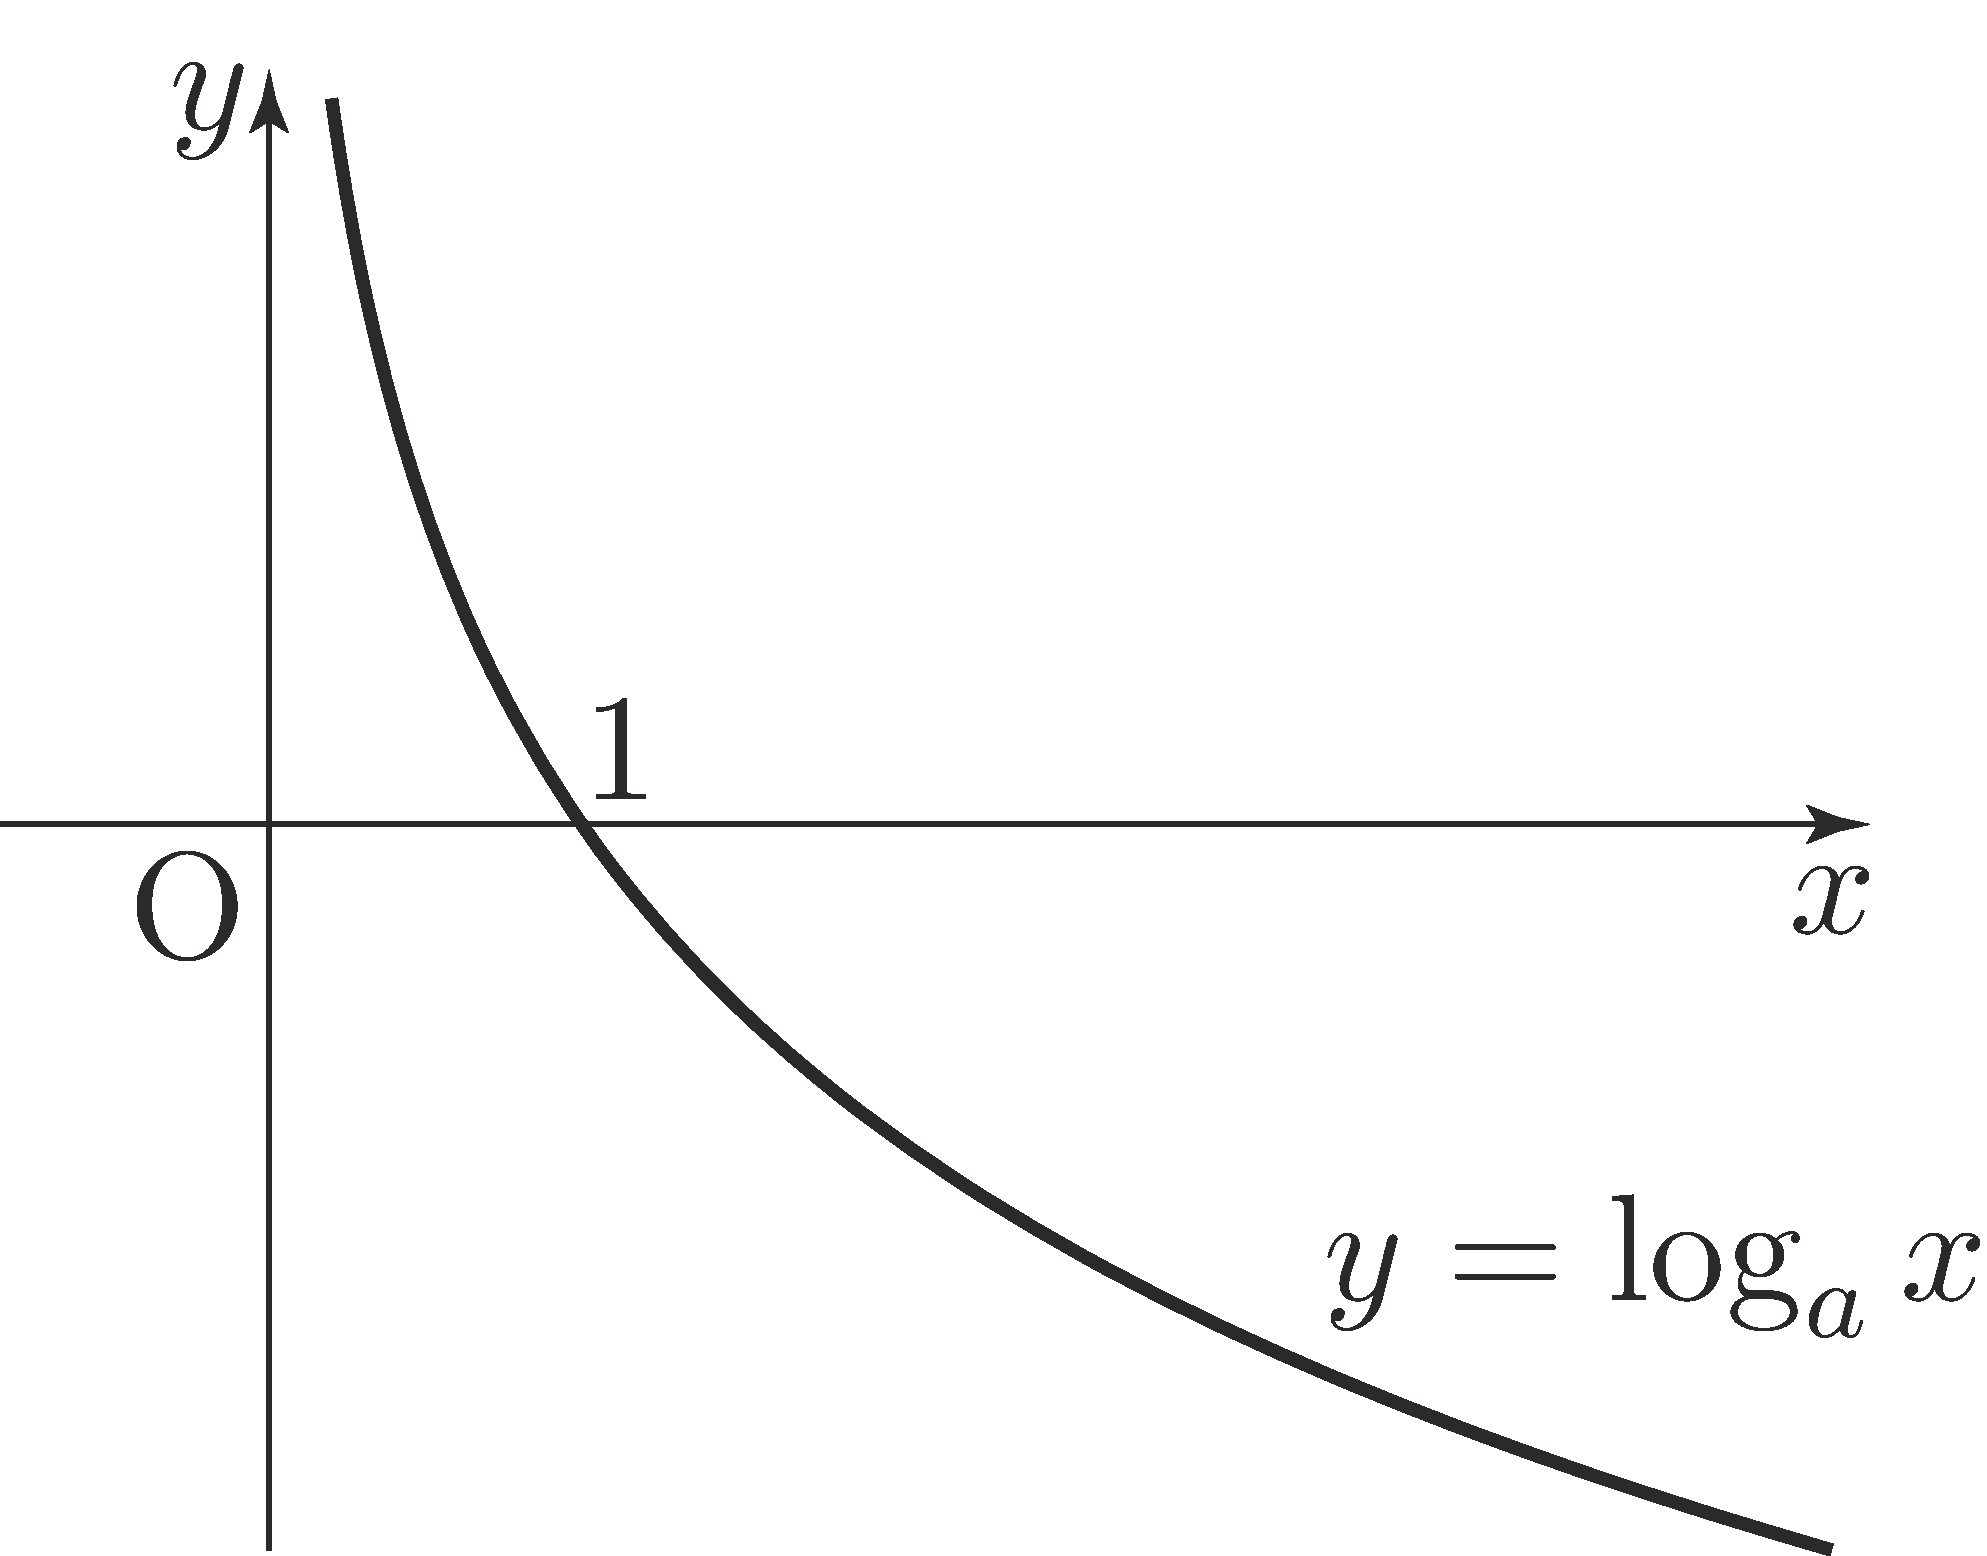
\includegraphics[scale=\pgfkeysvalueof{picsize}]{DBs/pic/zert_02_2.pdf}}\
	\end{figure}


로그함수 $y=\log_a x$에서 $x=1$을 대입하면 $a$의 값에 관계 없이 $y=0$이므로, 로그함수의 그래프는 $a$의 값에 관계 없이 $\xy{1}{0}$을 지납니다. $a>1$이면 (a)와 같고, $0<a<1$이면 (b)와 같습니다.

\begin{figure}[h]
	\centering \subfloat[][]{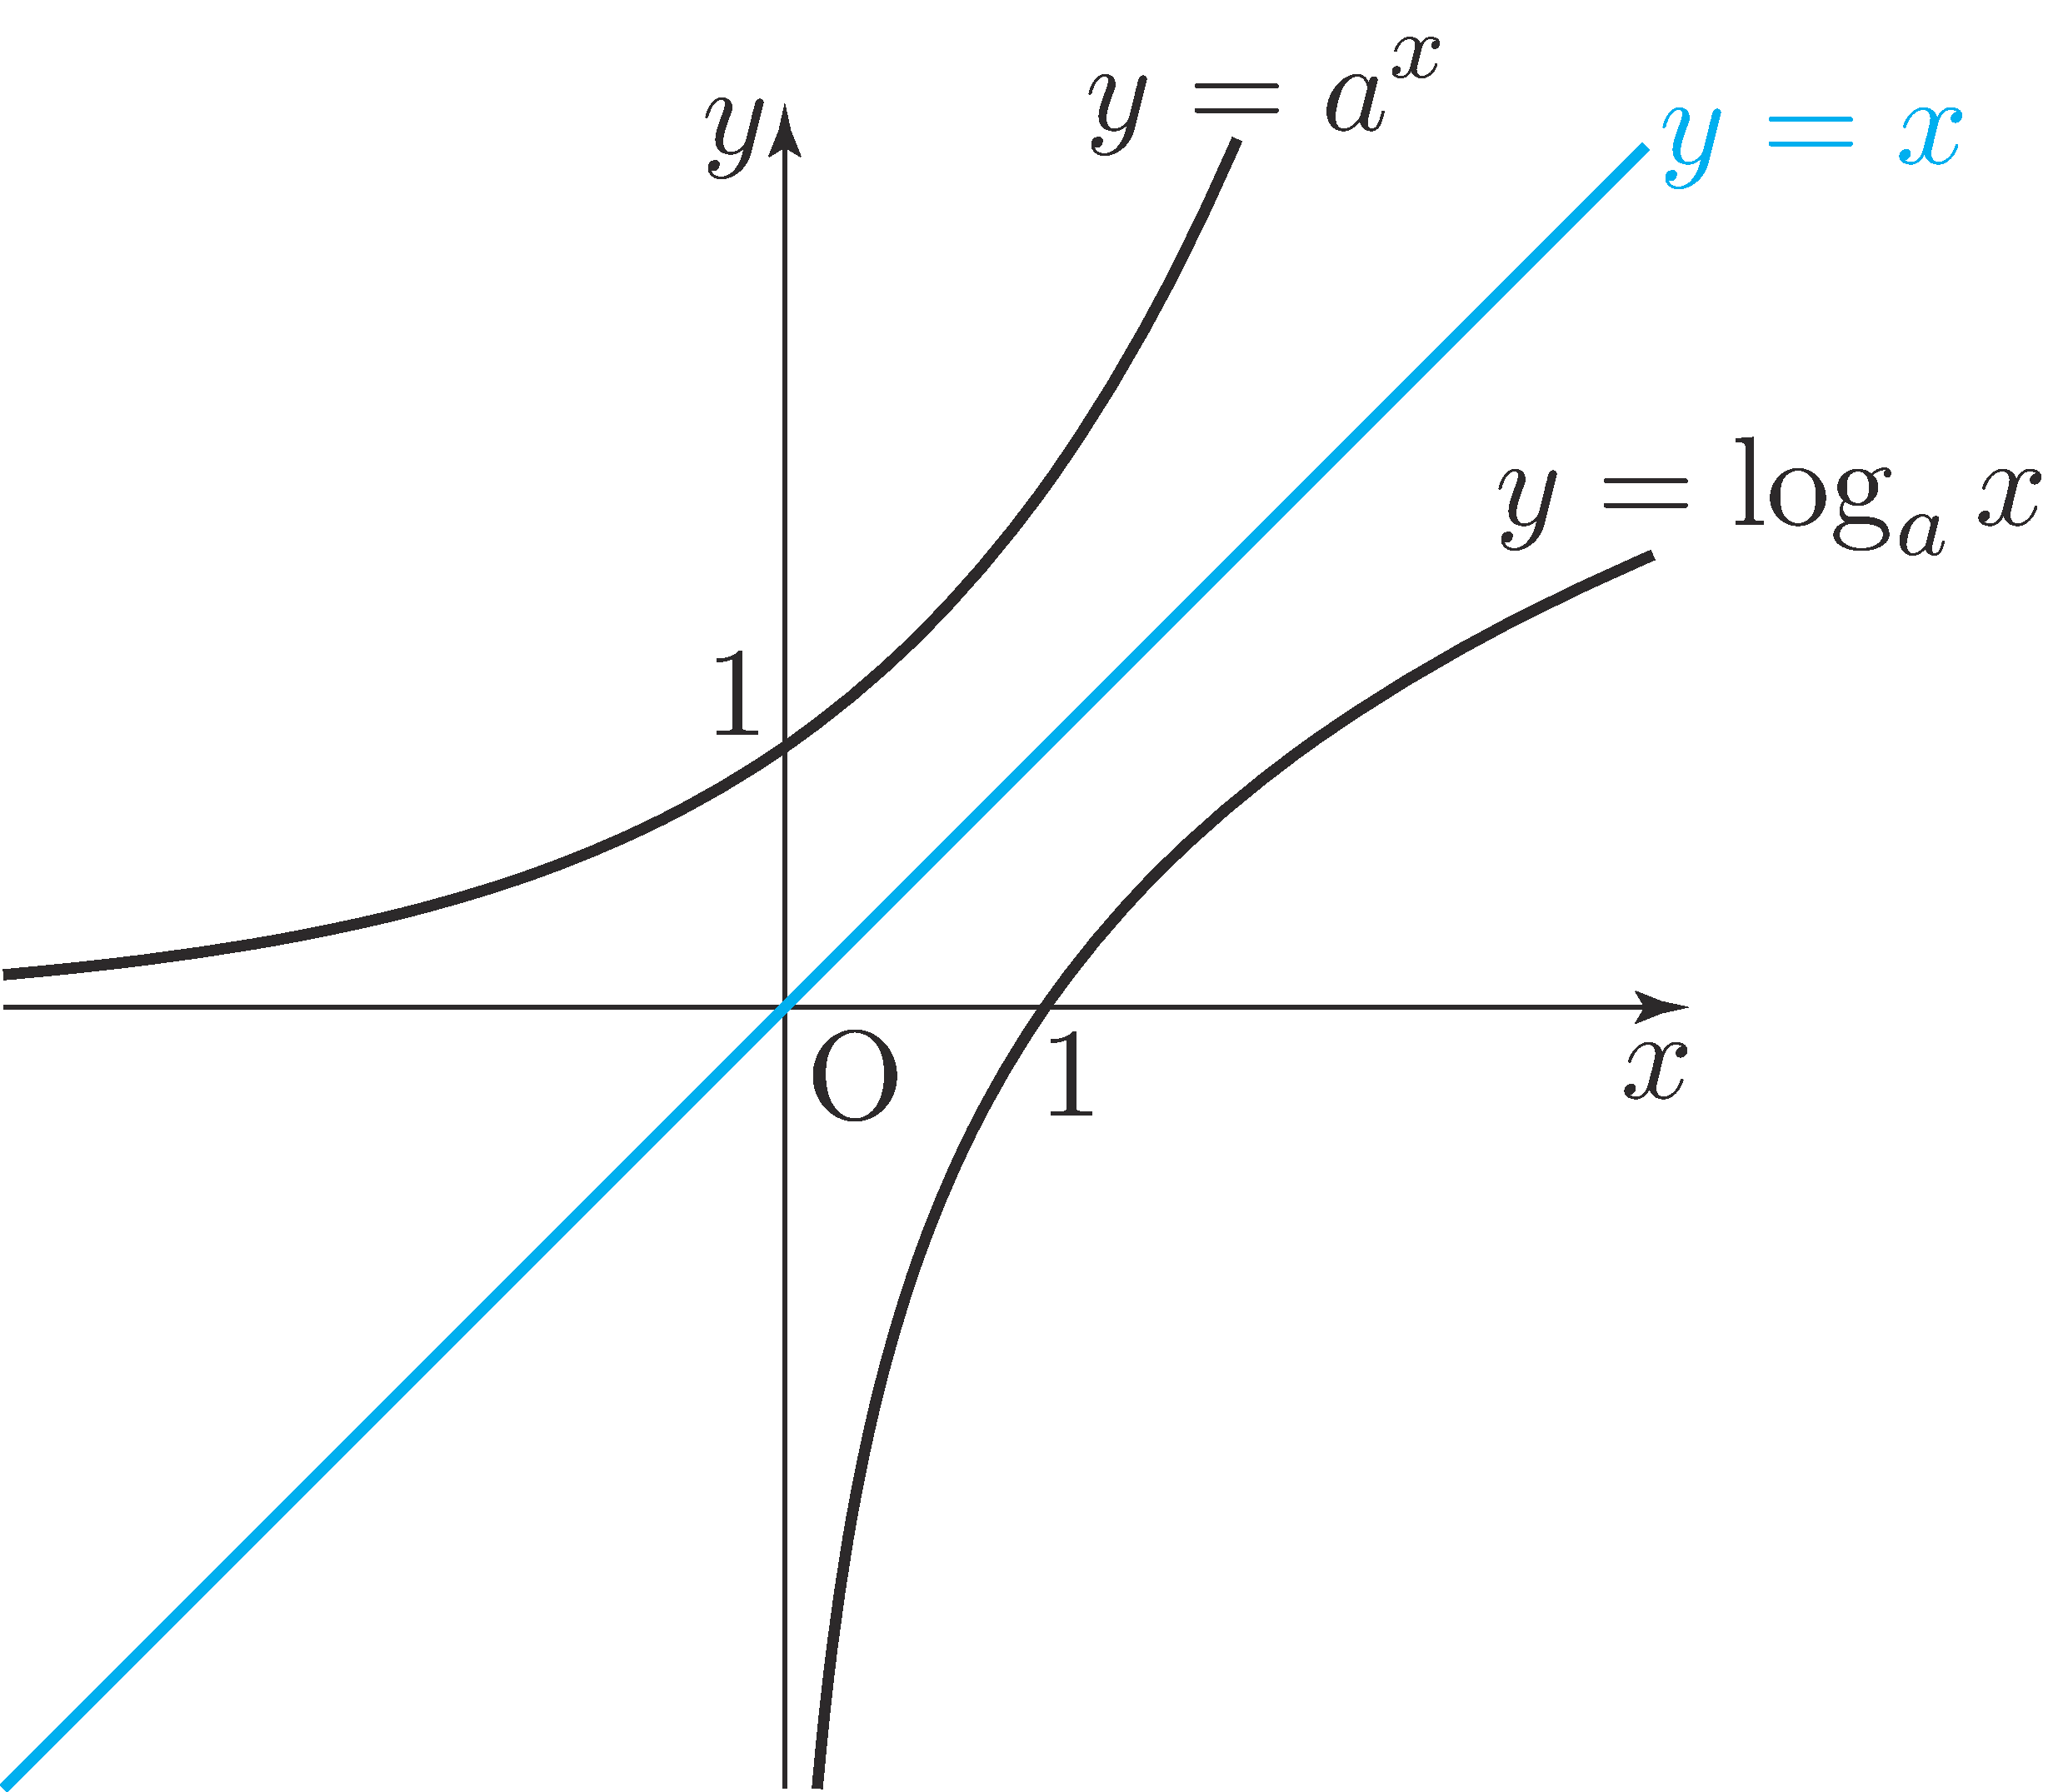
\includegraphics[scale=\pgfkeysvalueof{picsize}]{DBs/pic/zert_03_1.pdf}}\
	\qquad
	\centering \subfloat[][]{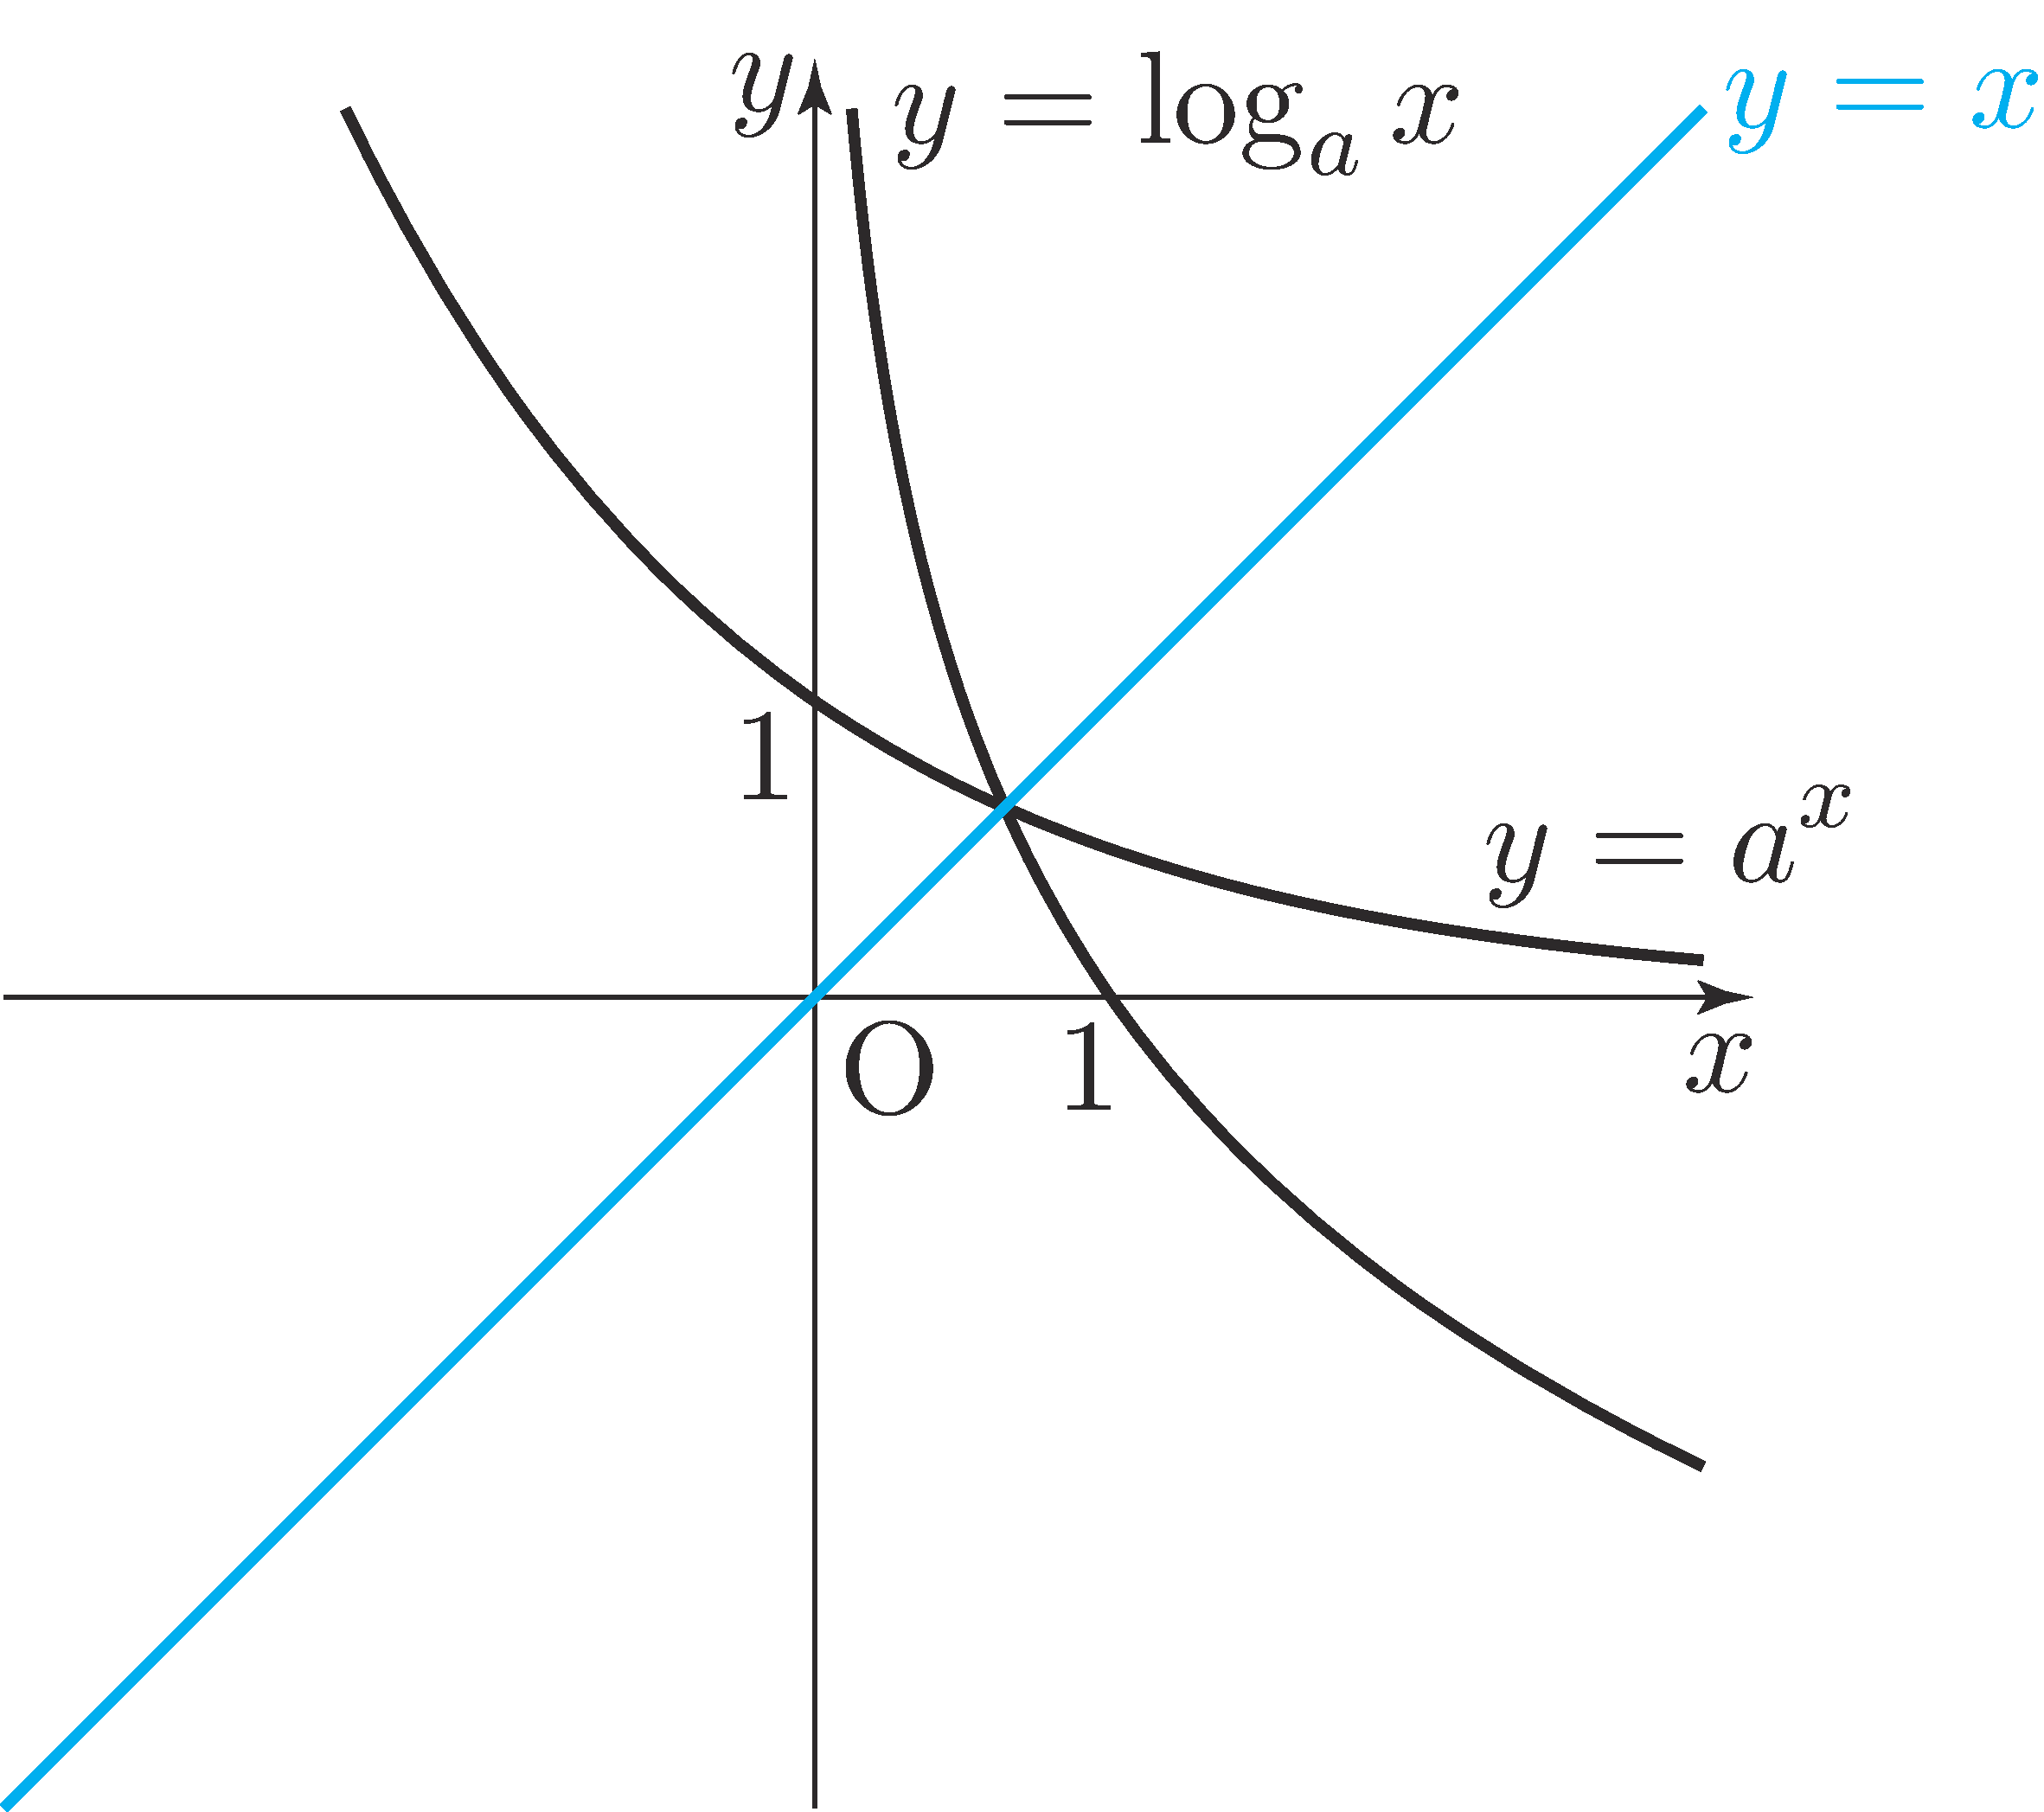
\includegraphics[scale=\pgfkeysvalueof{picsize}]{DBs/pic/zert_03_2.pdf}}\
	\end{figure}


지수함수와 로그함수는 서로 역함수 관계이므로 두 함수의 그래프는 직선 $y=x$에 대하여 대칭입니다. $a>1$이면 (a)와 같고, $0<a<1$이면 (b)와 같습니다.\mn[-5\blskip]{교과서에는 이 그림만 실려 있기 때문에 지수함수의 그래프와 로그함수의 그래프의 위치관계가 항상 이 두 그림 중 하나라고 생각하기 쉽습니다. 그러나 더 많은 위치관계가 존재합니다. 이는 Math I에서 다룹니다.}{}

\clearpage
\mychapter{공통 삼각함수}{}
\section{일반각}
$360^\circ$를 초과하거나 $0^\circ$ 미만인 각을 정의할 수 있습니다.
\begin{center}
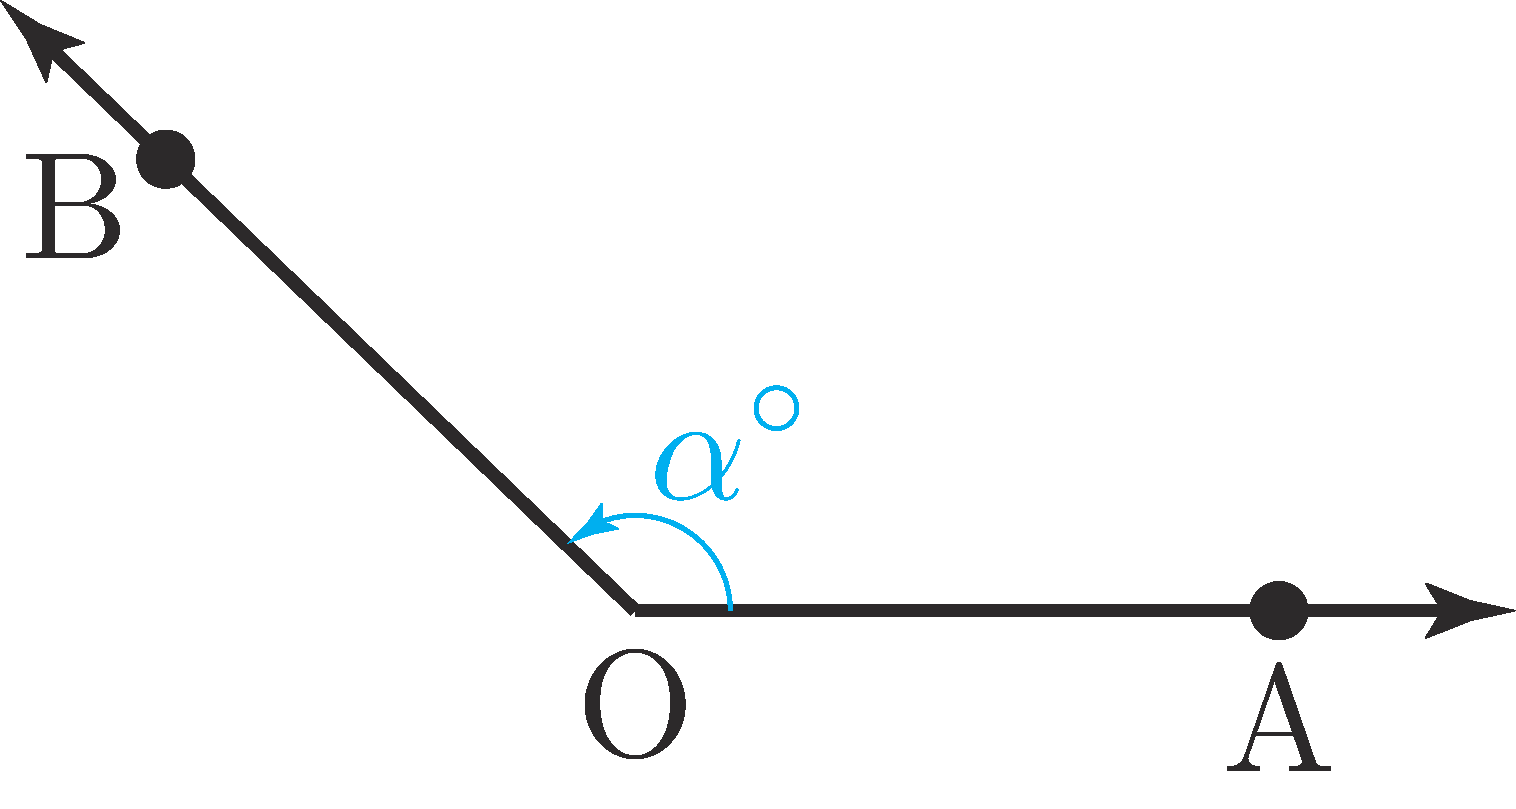
\includegraphics[scale=\pgfkeysvalueof{picsize}]{DBs/pic/zert_04.pdf}\
\end{center}$0 \le \alpha < 360$인 실수 $\alpha$에 대하여 각 $\mrm{AOB}$의 크기를 $\alpha^\circ$라 할 때, 각의 정의에 따르면 반직선 $\mrm{OA}$를 $\mrm{O}$를 중심으로 회전시켜 반직선 $\mrm{OB}$와 겹치게 할 수 있을 때 회전한 양이 $\alpha^\circ$입니다.
\begin{center}
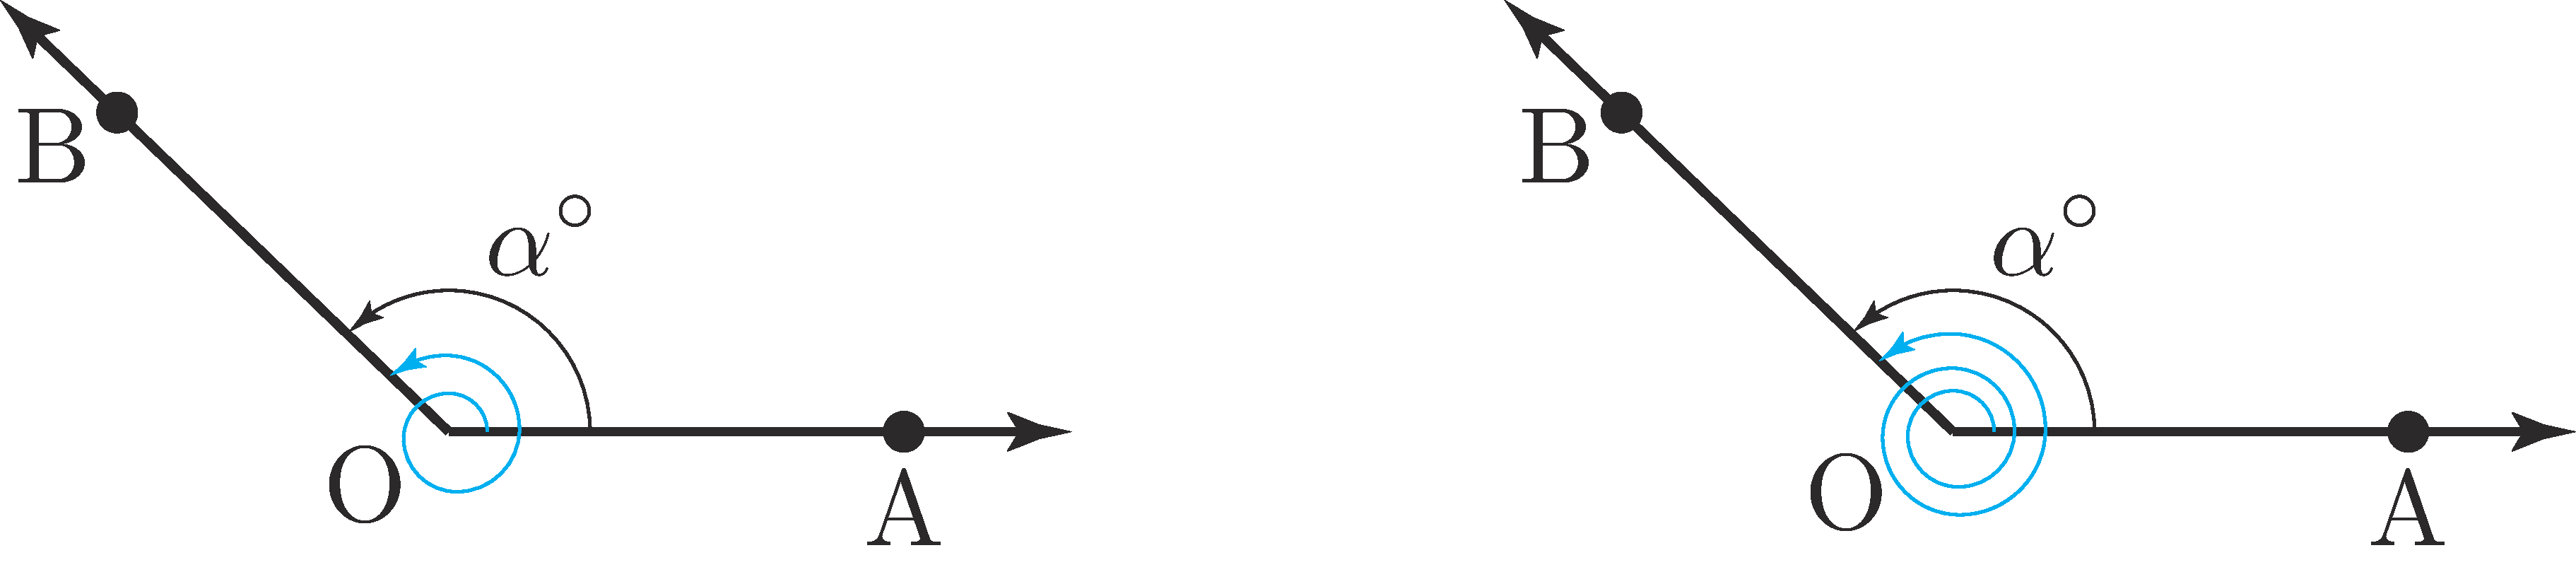
\includegraphics[scale=\pgfkeysvalueof{picsize}]{DBs/pic/zert_05.pdf}\
\end{center}그런데 $\alpha^\circ$만큼 회전한 후 같은 방향으로 한 바퀴를 더 돌아도, 즉 $\alpha^\circ + 360^\circ$만큼 회전하여도 반직선 $\mrm{OA}$를 반직선 $\mrm{OB}$와 겹치게 할 수 있습니다. 마찬가지로 모든 자연수 $n$에 대하여 $\alpha^\circ + n\times 360^\circ$만큼 회전하여도 반직선 $\mrm{OA}$를 반직선 $\mrm{OB}$와 겹치게 할 수 있습니다. 같은 방법으로 $\alpha^\circ$만큼 회전한 후 반대 방향으로 한 바퀴를 더 돌아도, 즉 $\alpha^\circ - 360^\circ$만큼 회전하여도 반직선 $\mrm{OA}$를 반직선 $\mrm{OB}$와 겹치게 할 수 있습니다. 마찬가지로 모든 자연수 $n$에 대하여 $\alpha^\circ - n\times 360^\circ$만큼 회전하여도 반직선 $\mrm{OA}$를 반직선 $\mrm{OB}$와 겹치게 할 수 있습니다.

이런 방법으로 모든 정수 $n$에 대하여 각 $\mrm{AOB}$의 크기를 $\alpha^\circ + n\times 360^\circ$라 나타낼 수 있습니다. 이때 시계 반대 방향으로 회전하는 것을 양의 방향 $(+)$, 시계 방향으로 회전하는 것을 음의 방향 $(-)$이라 하고, 이렇게 확장된 각의 정의를 \term{일반각}{}이라 합니다.

\section{호도법}
\begin{center} 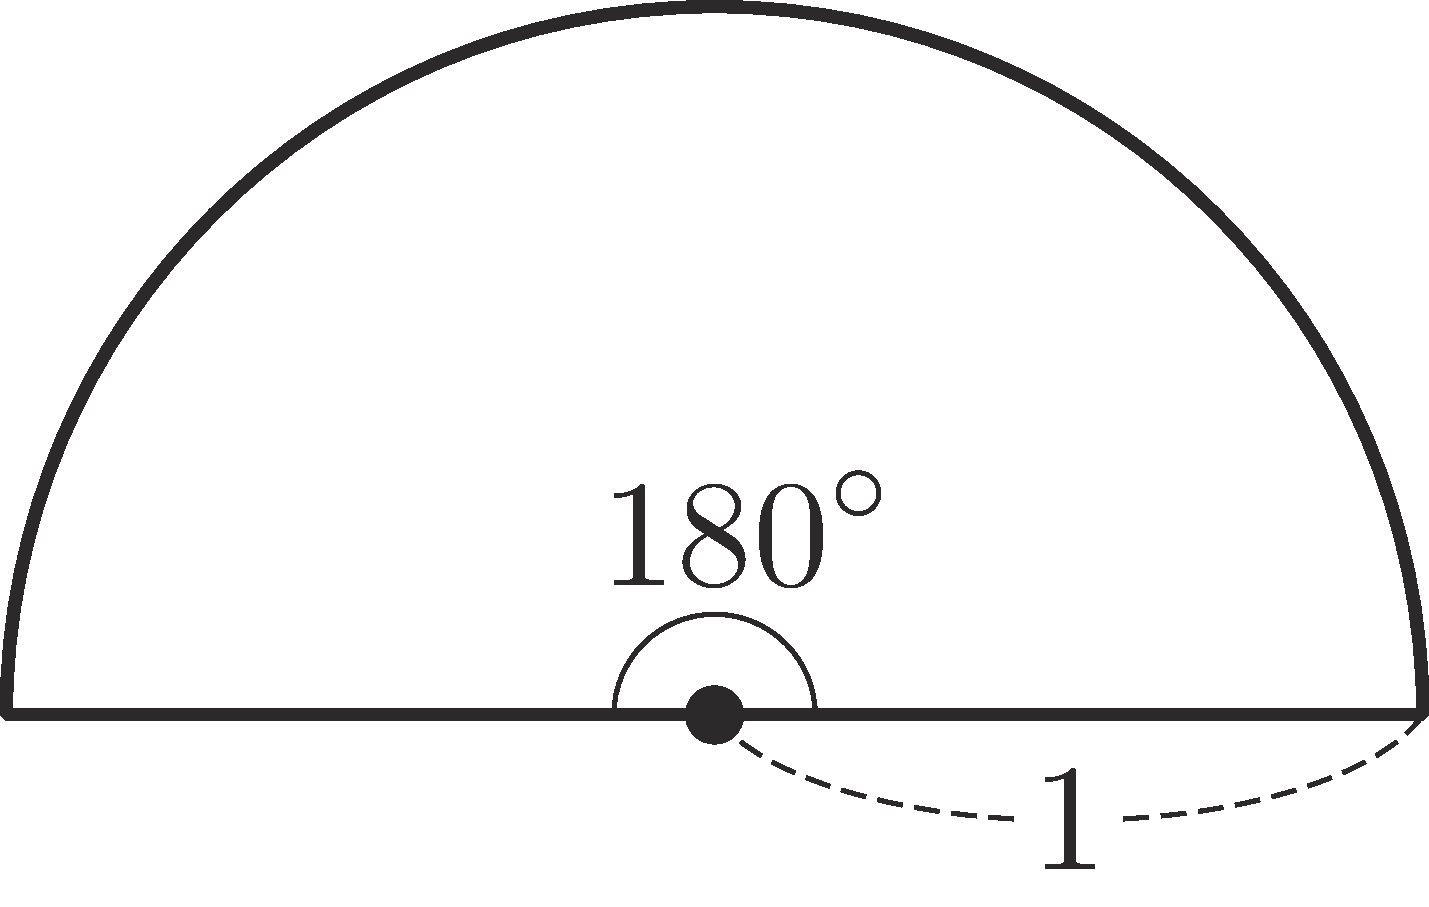
\includegraphics[scale=\pgfkeysvalueof{picsize}]{DBs/pic/zert_06.pdf}\
	\end{center}부채꼴에서 호의 길이는 중심각과 정비례하므로, 호의 길이를 이용하여 각도를 표시하는 단위를 생각할 수 있습니다. 반지름이 $1$이고 중심각이 $180^\circ$인 부채꼴, 즉 반원의 호의 길이는 $\pi$입니다. 이때 이 `호의 길이'를 그대로 `각의 크기'로 사용하는, 즉 `반원의 중심각은 $\pi$'와 같이 호의 길이를 각도의 크기에 대응시키는 방법이 \term{호도법}{}입니다.

호도법에서의 각도의 단위를 \term{라디안}{}이라 합니다. 호도법을 쓸 때에는 일반적으로 단위인 `라디안'을 생략하고 적습니다. 호도법을 이용하여 자주 사용되는 각의 크기를 나타내면 $30^\circ = \dfrac{\pi}{6}$, $45^\circ=\dfrac{\pi}{4}$, $60^\circ = \dfrac{\pi}{3}$, $90^\circ=\dfrac{\pi}{2}$, $360^\circ=2\pi$와 같습니다. 
\begin{center} 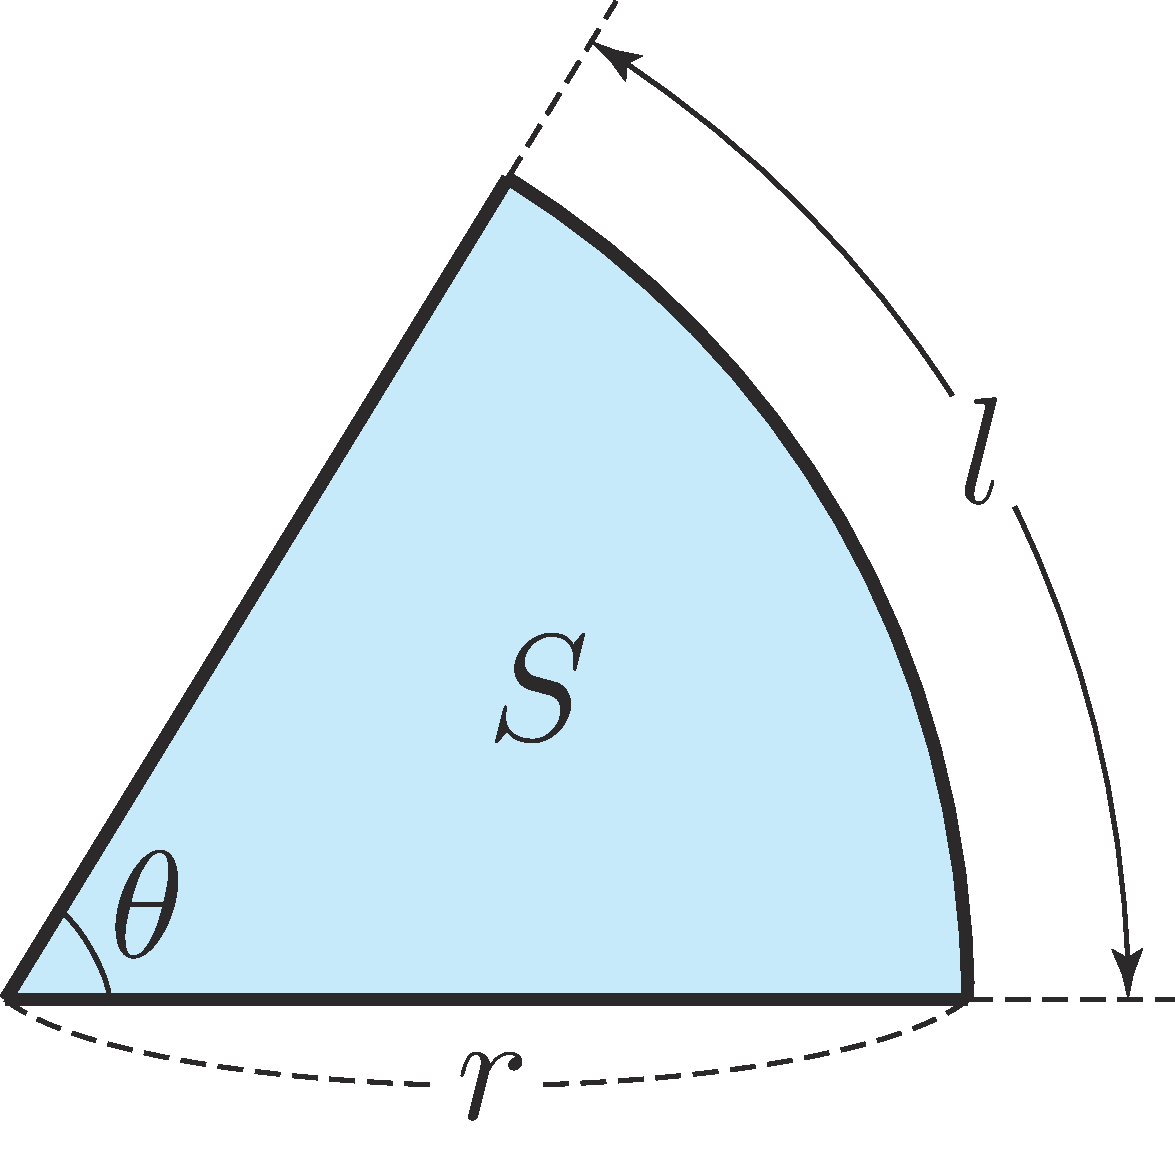
\includegraphics[scale=\pgfkeysvalueof{picsize}]{DBs/pic/zert_07.pdf}\
	\end{center}호도법을 이용하면 호의 길이, 부채꼴의 넓이를 구할 때 $\dfrac{\text{중심각의 크기}^\circ}{360^\circ}$를 사용하지 않고 쉽게 구할 수 있습니다. 예를 들어 중심각의 크기가 $\theta$이고 반지름의 길이가 $r$인 부채꼴에서 호의 길이 $l$에 대하여 $l = r\theta$입니다. 또한 부채꼴의 넓이 $S$에 대하여 $S = \dfrac{1}{2}lr$이므로 $l = r\theta$를 대입하면 $S =\dfrac{1}{2}r^2\theta$입니다.\\[-2em]

\section{삼각비}
\begin{center}
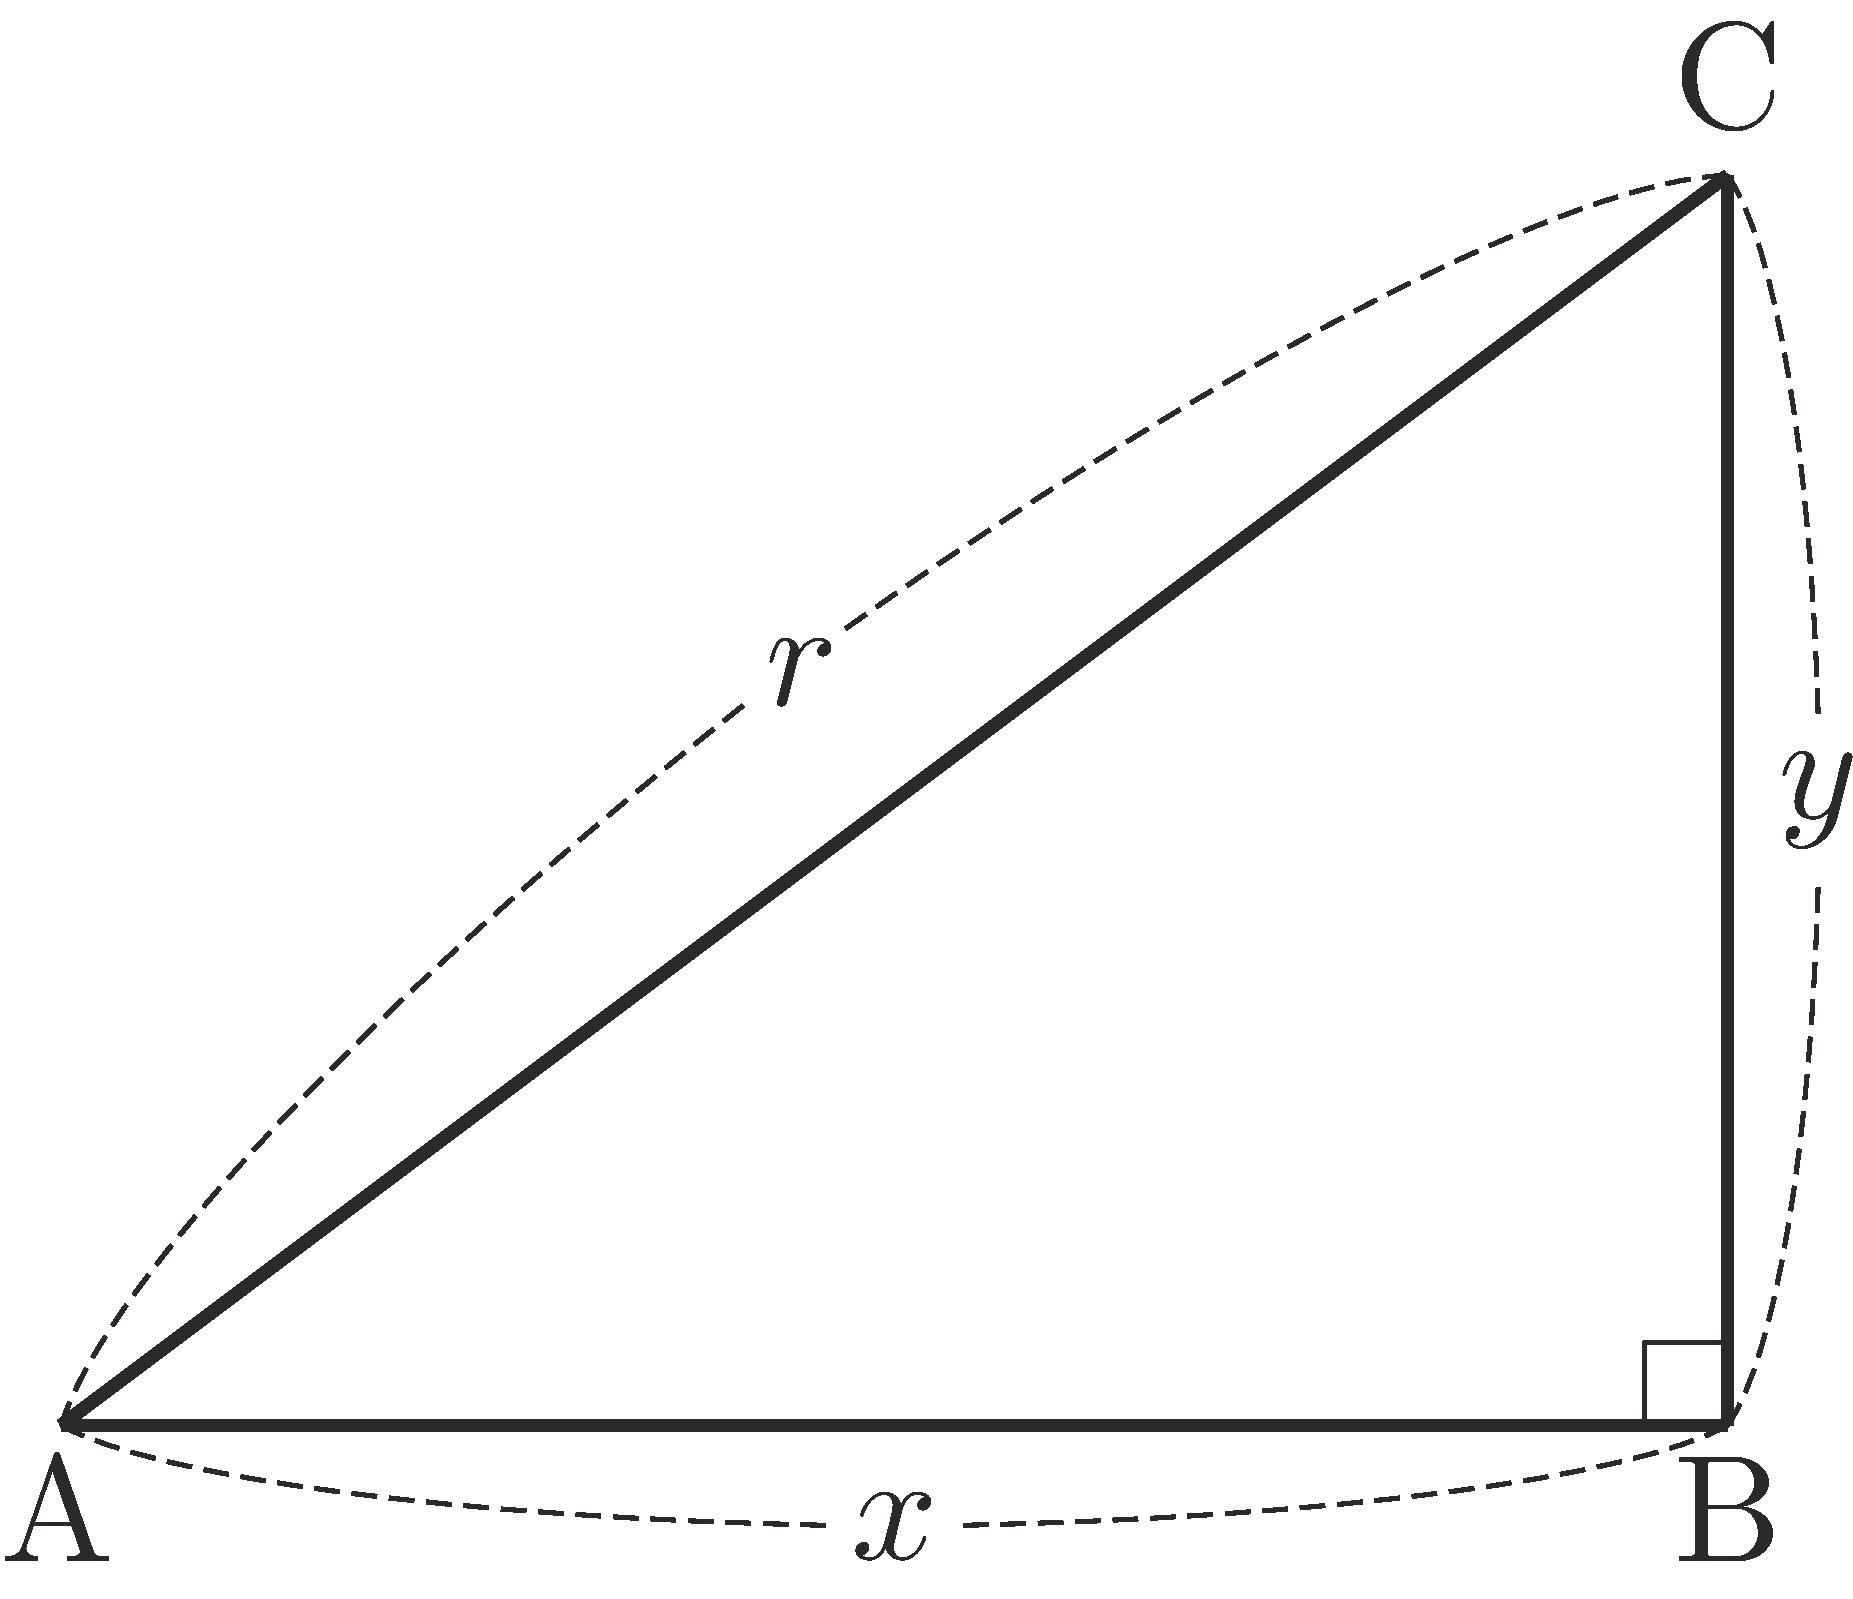
\includegraphics[scale=0.125]{pic0/pic154.pdf}
\end{center}$\angle \mrm{B} = 90^\circ$이고 $\ovr{AC}=r$, $\ovr{AB}=x$, $\ovr{BC}=y$인 직각삼각형 $\mrm{ABC}$에서 $\angle \mrm{A}$에 대한 \term{삼각비}{}인 \term{사인}{2}, \term{코사인}{}, \term{탄젠트}{}를 다음과 같이 정의합니다.
\begin{align*} 
\sin \angle \mrm{A} = \dfrac{y}{r},\quad
\cos \angle \mrm{A} = \dfrac{x}{r},\quad
\tan \angle \mrm{A} = \dfrac{y}{x} 
\end{align*}

\section{삼각함수}
\begin{center}
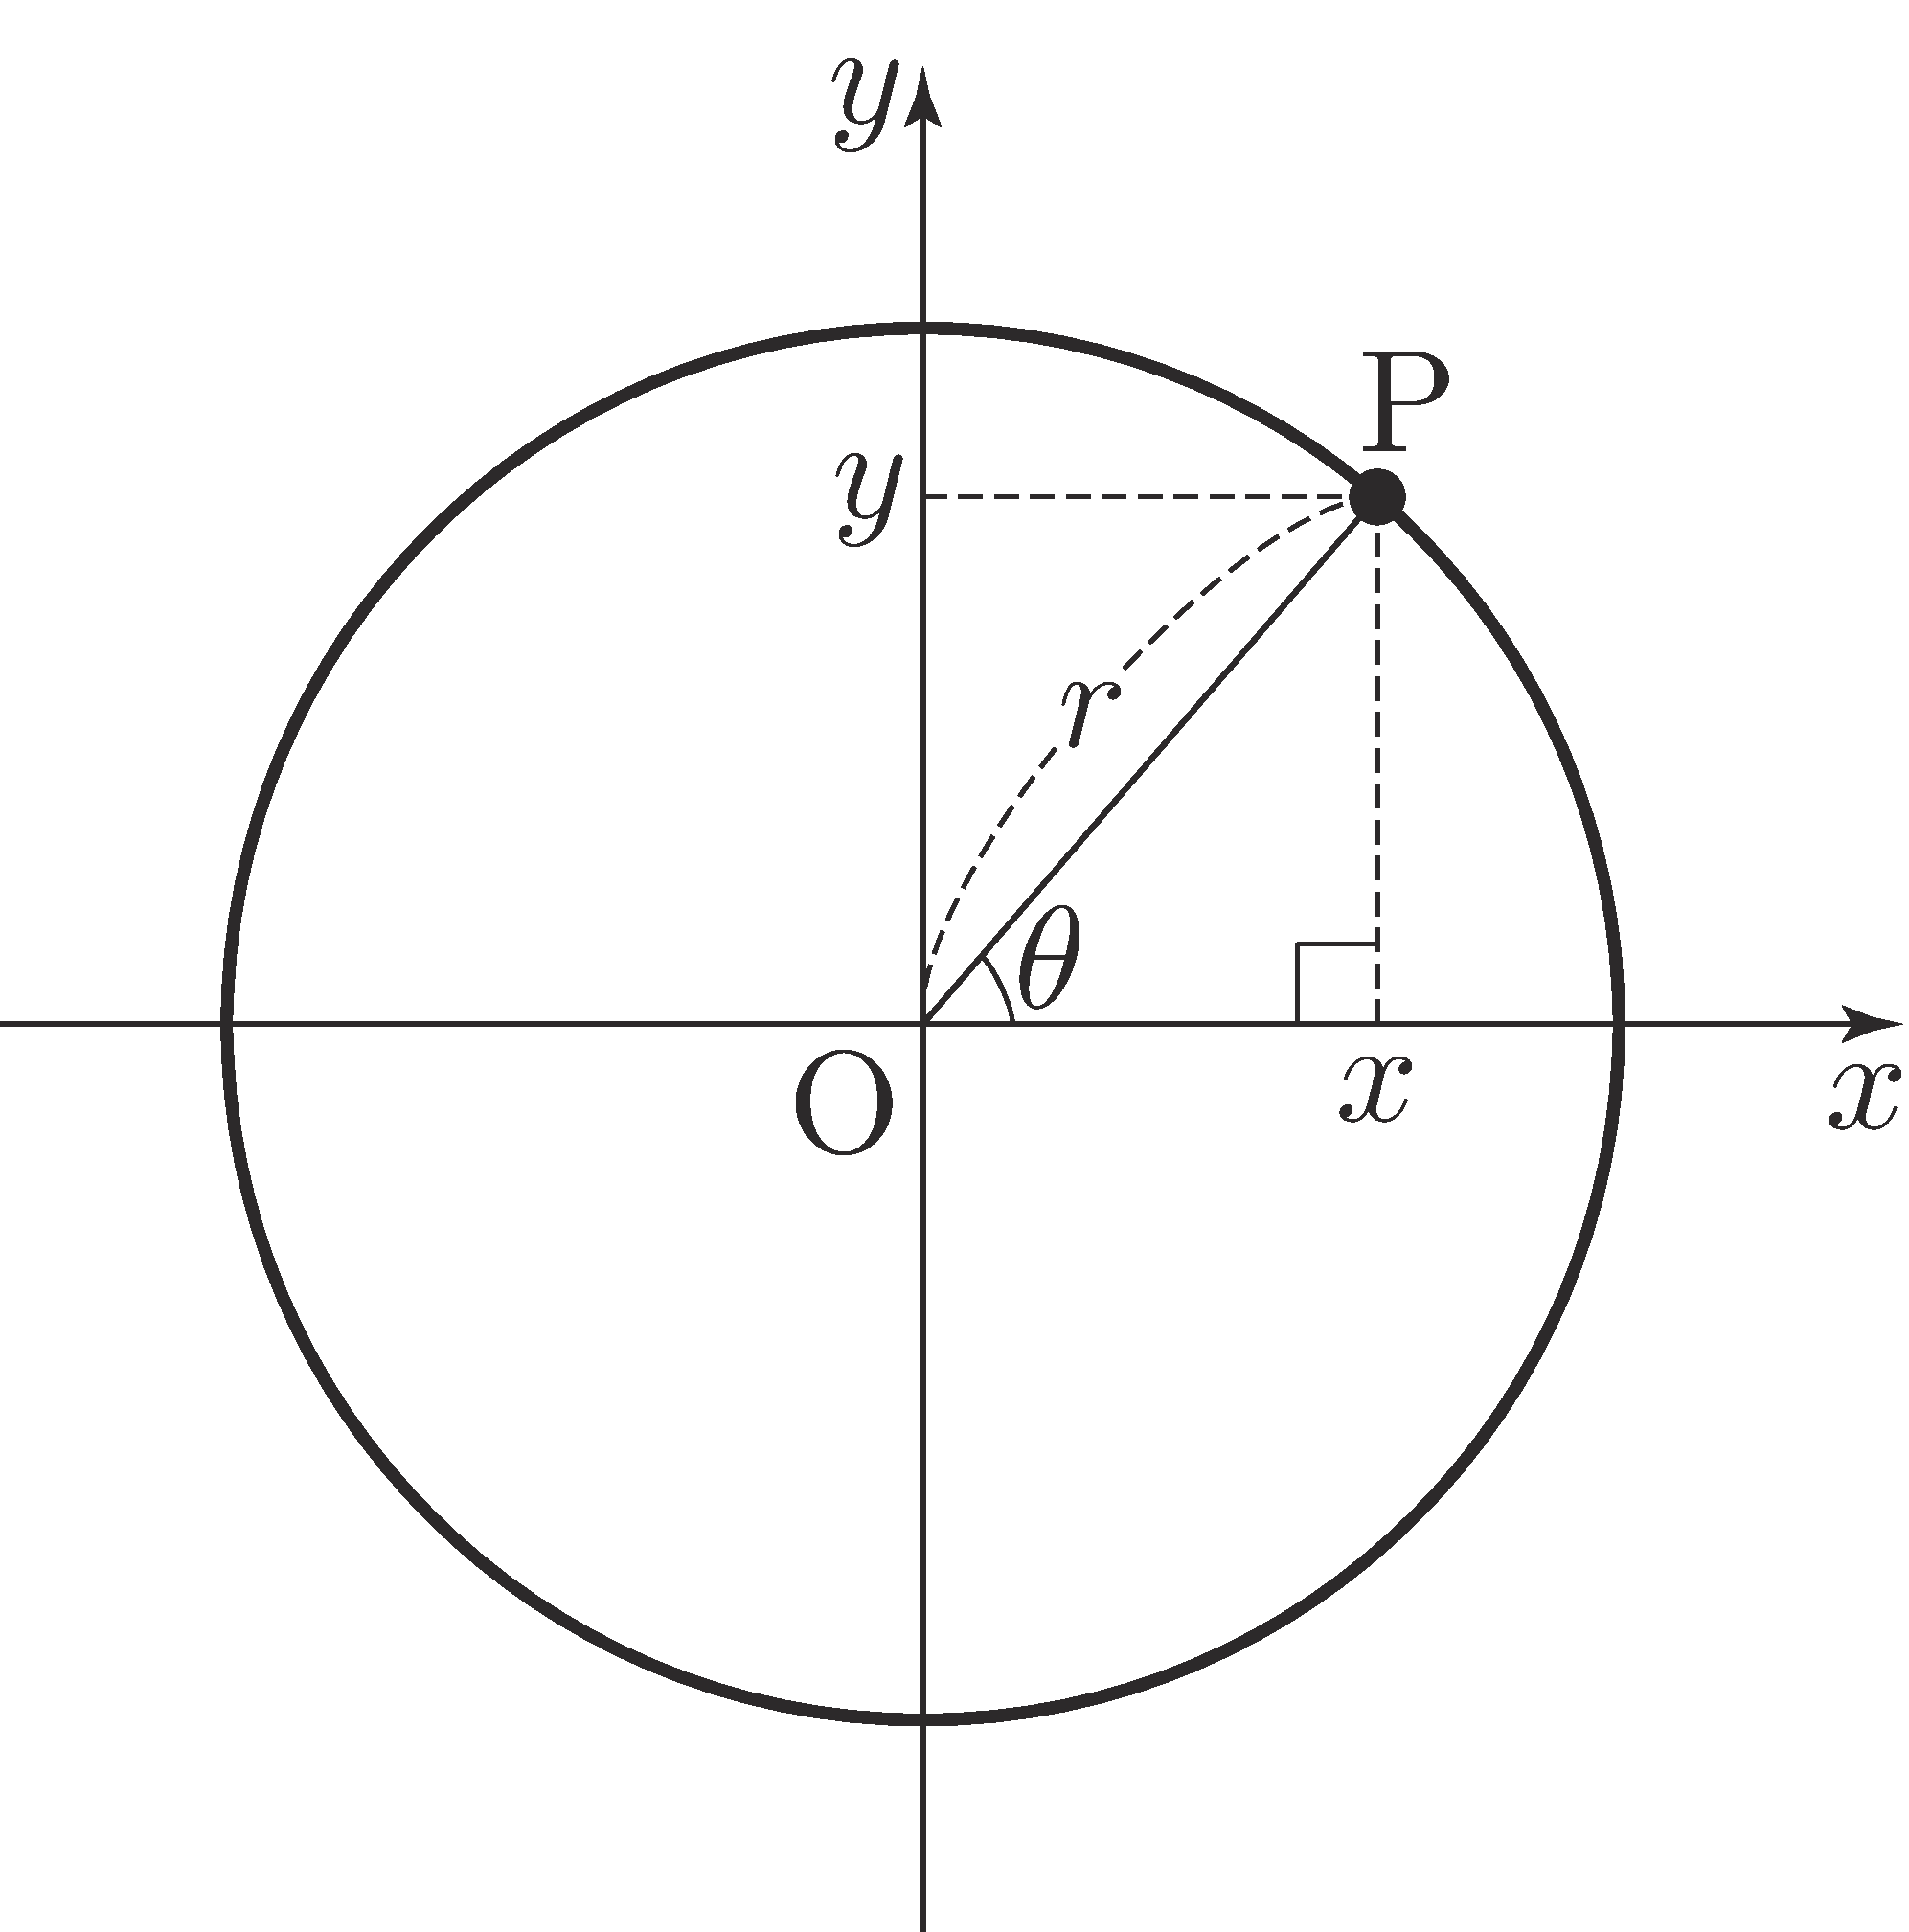
\includegraphics[scale=0.125]{pic0/pic155.pdf}
\end{center}좌표평면에서 중심이 원점 $\mrm{O}$이고 반지름의 길이가 $r$인 원 위의 점 $\xy[P]{x}{y}$에 대하여 직선 $\mrm{OP}$와 $x$축이 이루는 일반각을 $\theta$라 할 때, $\theta$에 대한 \term{삼각함수}{}인 \term{사인함수}{}, \term{코사인함수}{}, \term{탄젠트함수}{}를 다음과 같이 정의합니다.\mn{이때 $x$가 분모에 들어갈 때에는 $0$이 아니어야 합니다.}{}
\begin{align*}
  \sin \theta = \dfrac{y}{r},\quad
  \cos \theta = \dfrac{x}{r},\quad
  \tan \theta = \dfrac{y}{x}
\end{align*}
\clearpage
\subsection{삼각함수 사이의 관계}\term[삼각함수]{삼각함수 사이의 관계}{0}
$\tan\theta =\dfrac{y}{x} = \dfrac{\qfrac{y}{r}}{\qfrac*{x}{r}} =\dfrac{\sin\theta}{\cos\theta}$이므로 $\tan\theta=\dfrac{\sin\theta}{\cos\theta}$가 성립합니다. 한편 $\sin^2 \theta + \cos^2 \theta = \dfrac{x^2+y^2}{r^2} = 1$이므로 $\sin^2 \theta + \cos^2 \theta = 1$이 성립합니다.

\subsection{사인함수, 코사인함수, 탄젠트함수의 그래프}
\begin{center}
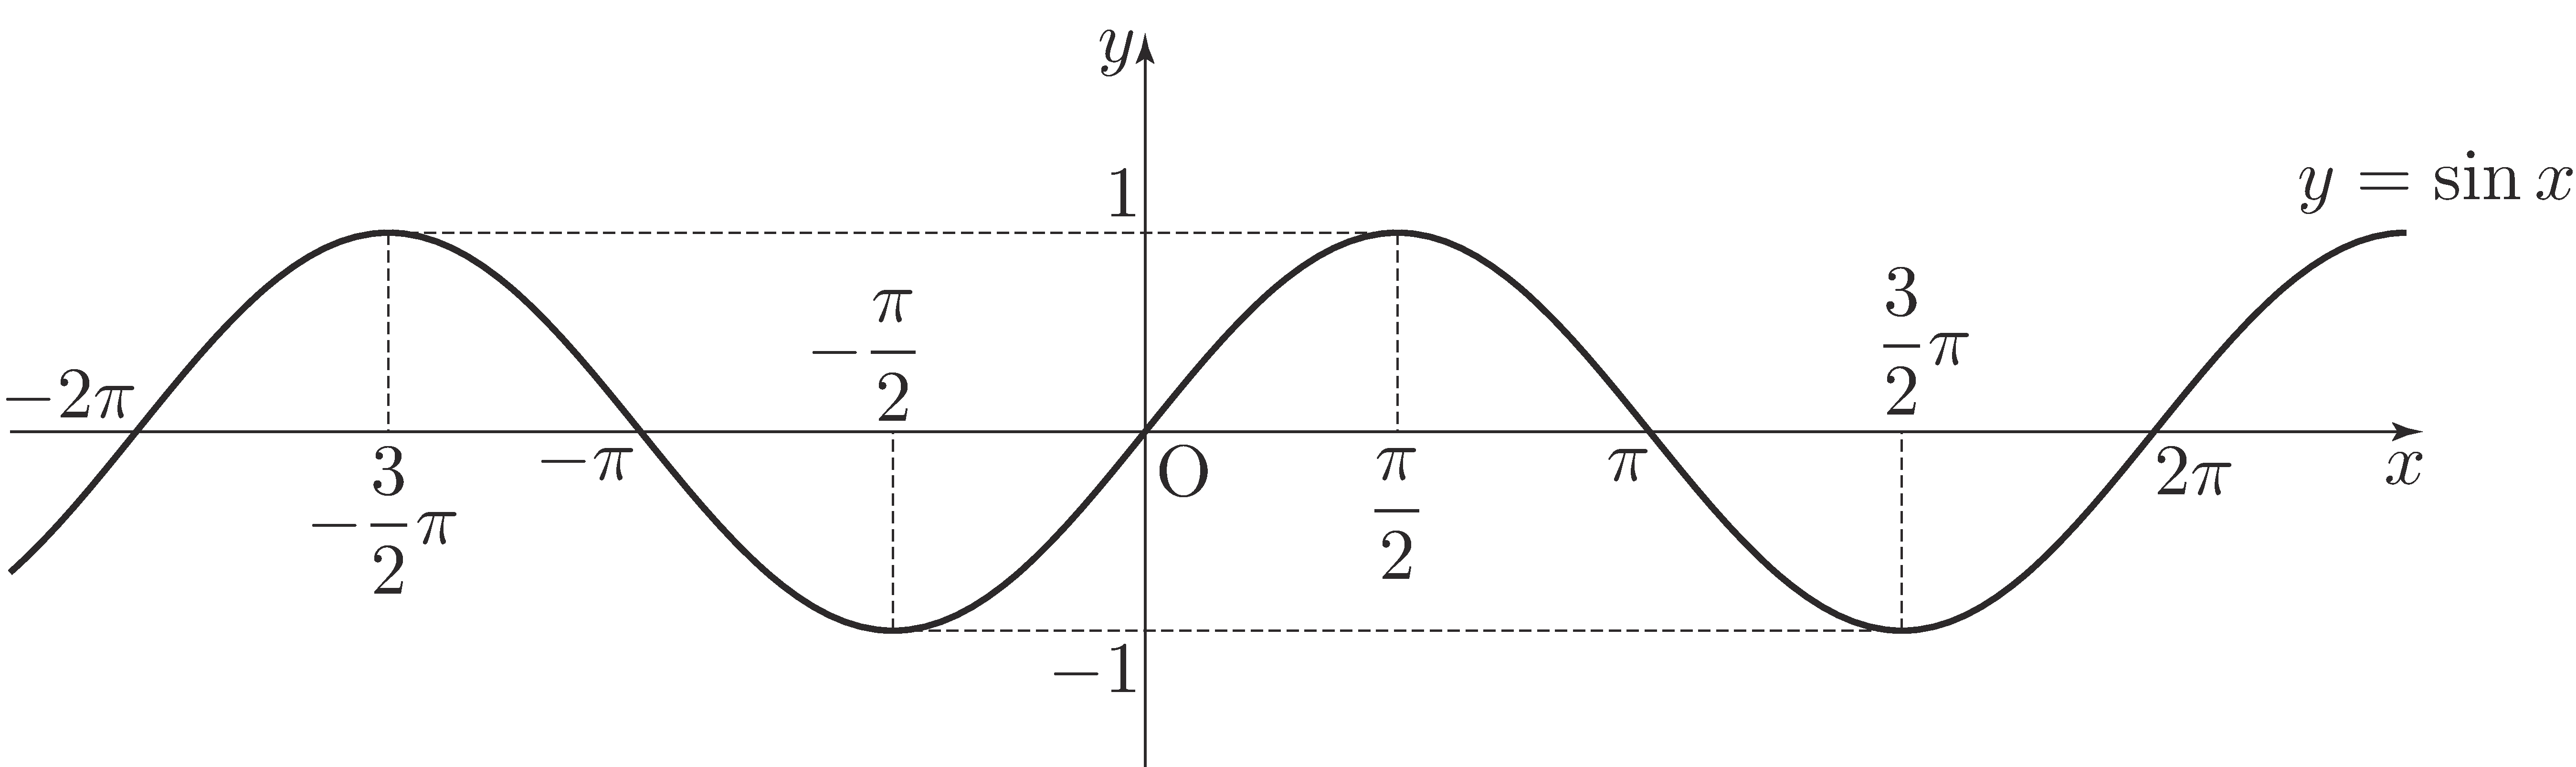
\includegraphics[scale=0.125]{pic0/pic156.pdf}
\end{center}사인함수 $y=\sin x$의 그래프는 위 그림과 같고, 원점에 대하여 대칭이며, 주기가 $2\pi$입니다.\term[사인함수]{사인함수의 그래프}{0}\mn{대칭, 주기 등의 용어에 대한 설명은 Graph에서 다룹니다.}{}
\begin{center}
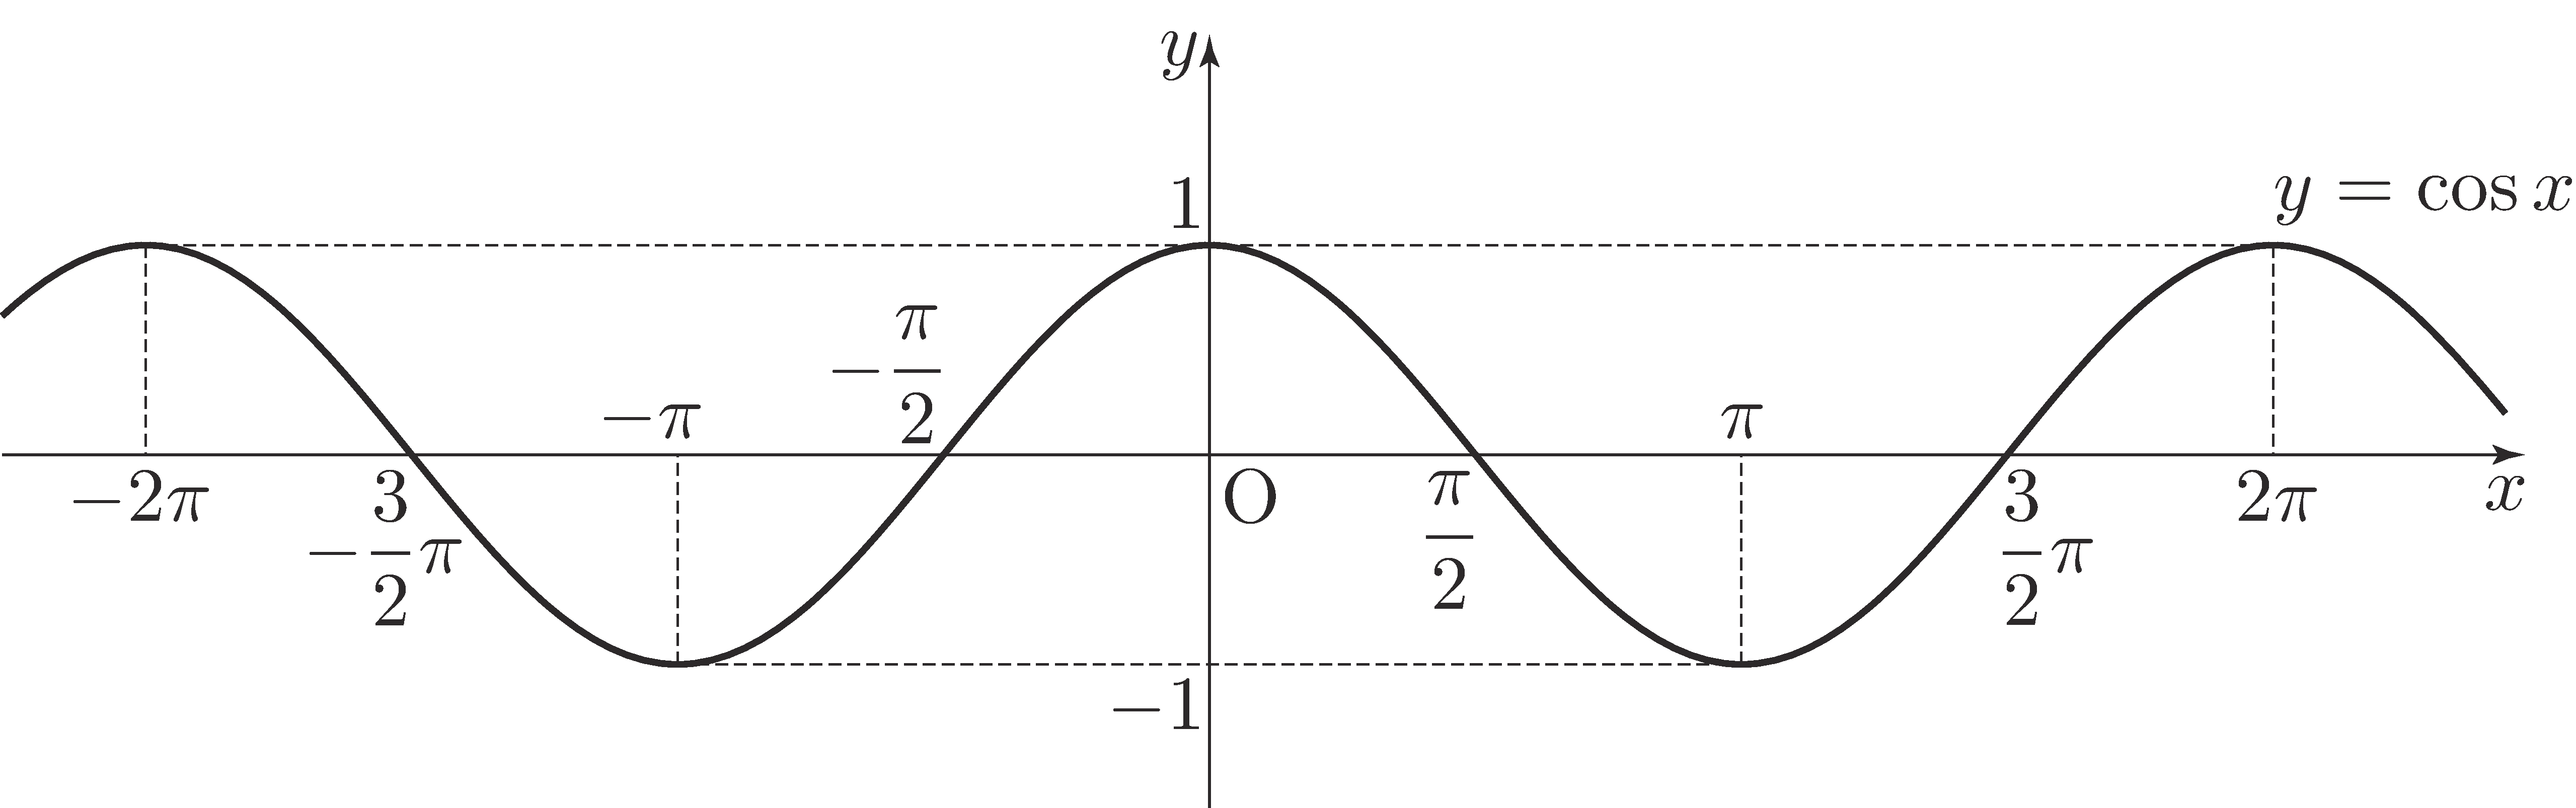
\includegraphics[scale=0.125]{pic0/pic157.pdf}
\end{center}코사인함수 $y=\cos x$의 그래프는 위 그림과 같고, $y$축에 대하여 대칭이며, 주기가 $2\pi$입니다.\term[코사인함수]{코사인함수의 그래프}{0}
\begin{center}
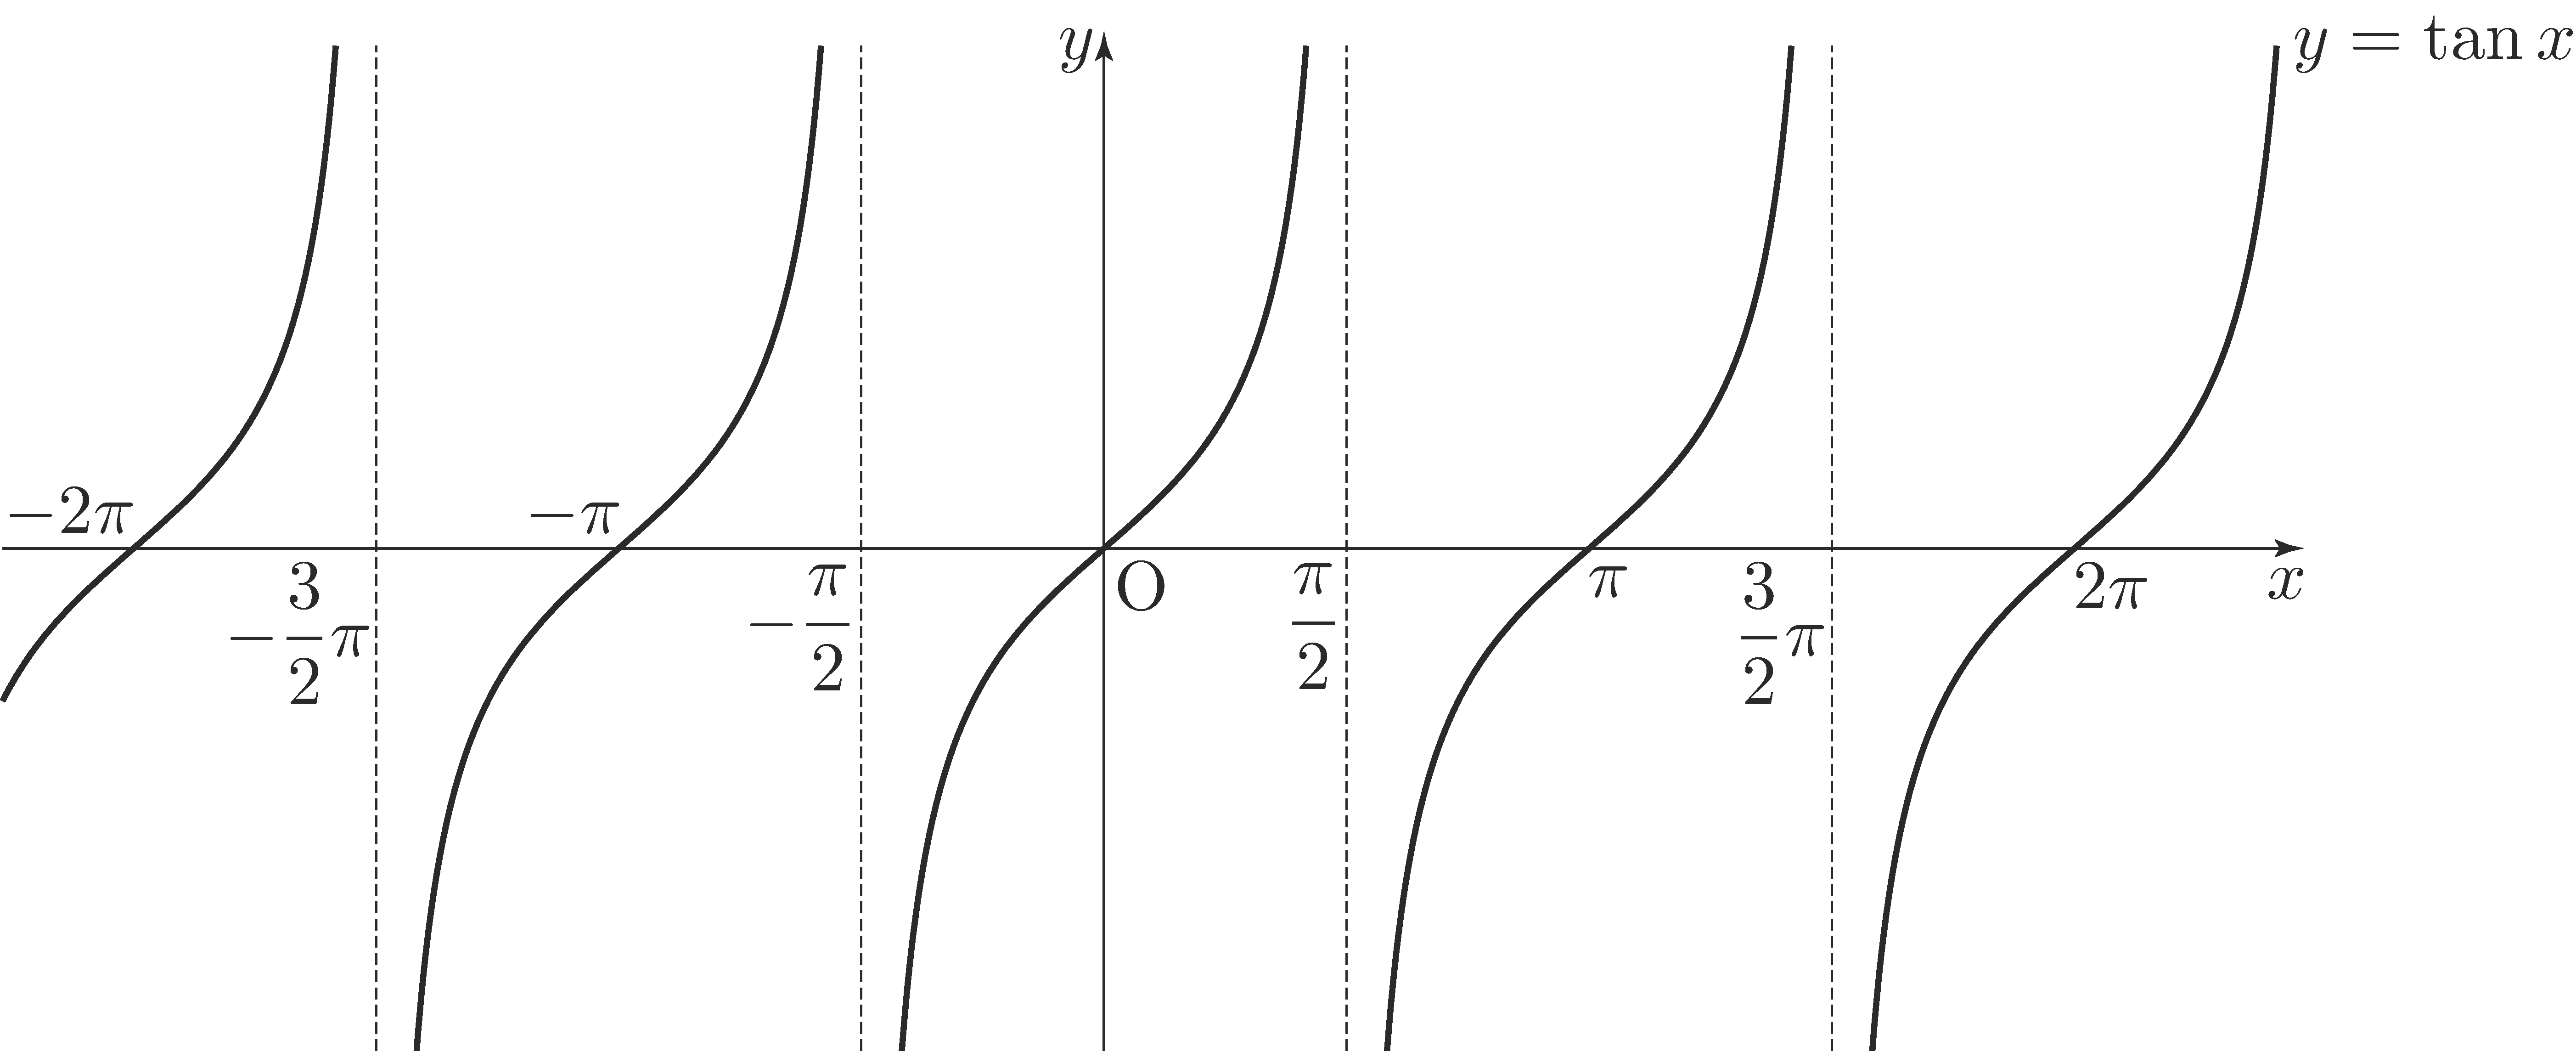
\includegraphics[scale=0.125]{pic0/pic158.pdf}
\end{center}탄젠트함수 $y=\tan x$의 그래프는 위 그림과 같고, 원점에 대하여 대칭이며, 주기가 $\pi$입니다.\term[탄젠트함수]{탄젠트함수의 그래프}{0}
\clearpage
\section{삼각함수의 활용}\term[선분!선분의 길이]{삼각함수를 이용하기}{0}
\subsection{선분의 길이를 삼각함수를 이용하여 나타내기}
\begin{center}
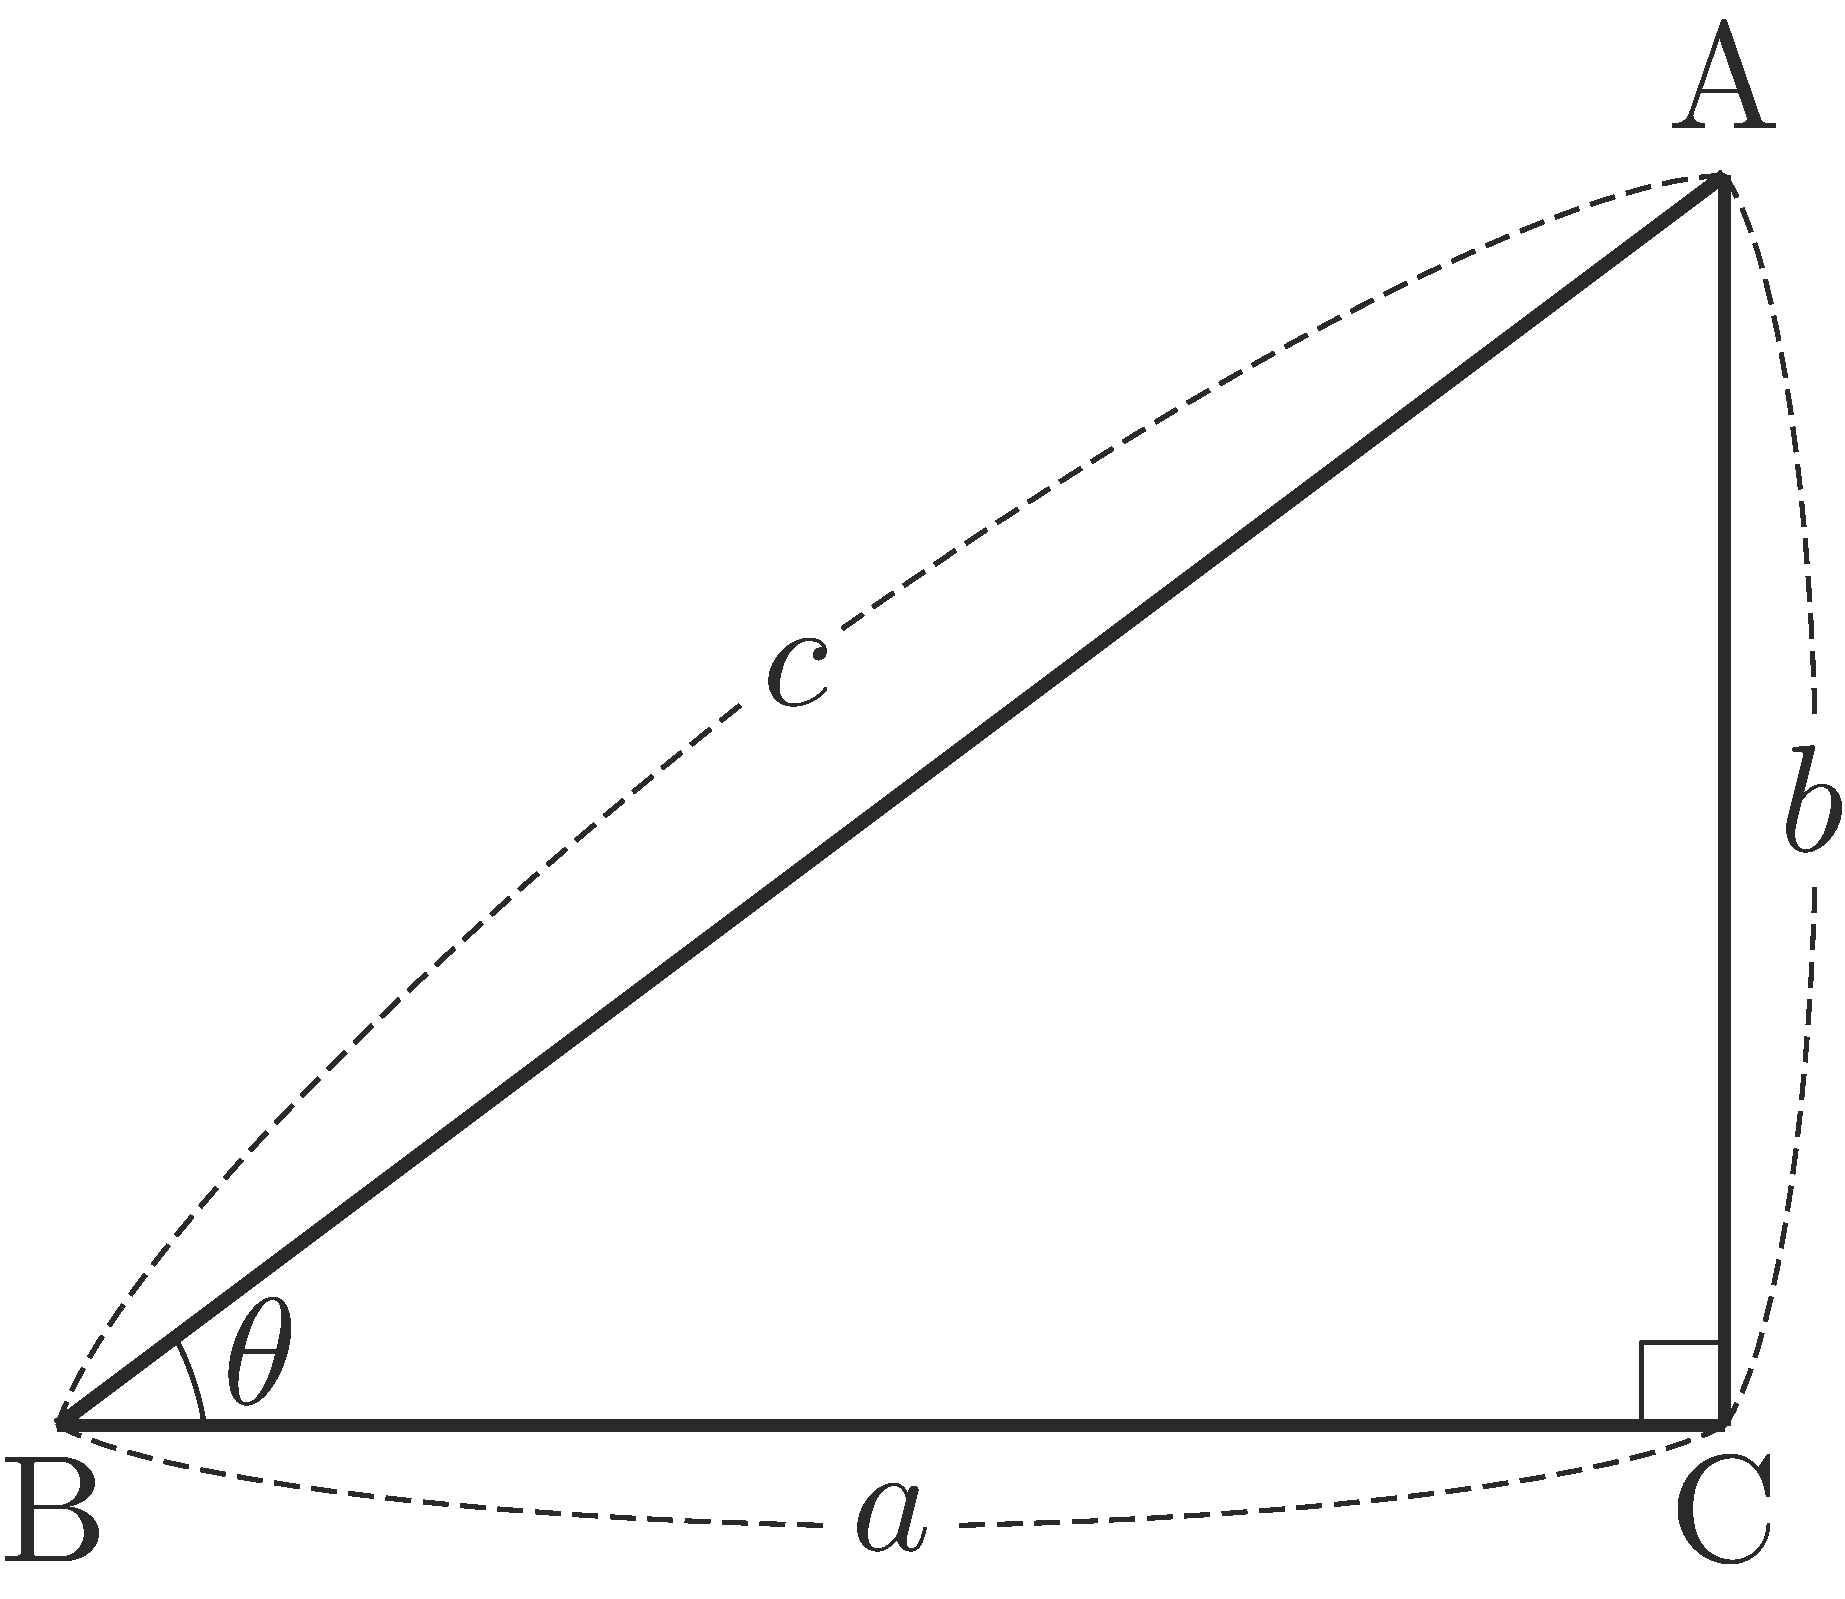
\includegraphics[scale=0.125]{pic0/pic159.pdf}
\end{center}그림과 같이 $\angle \mrm{C} = \dfrac{\pi}{2}$, $\angle \mrm{B} = \theta$인 직각삼각형에서 $a = c\times \cos\theta$, $b = c\times \sin\theta$, $b = a\times\tan\theta$ 등과 같이 선분의 길이를 삼각함수를 이용하여 나타낼 수 있습니다.

\subsection{사인법칙}\begin{center}  \centering 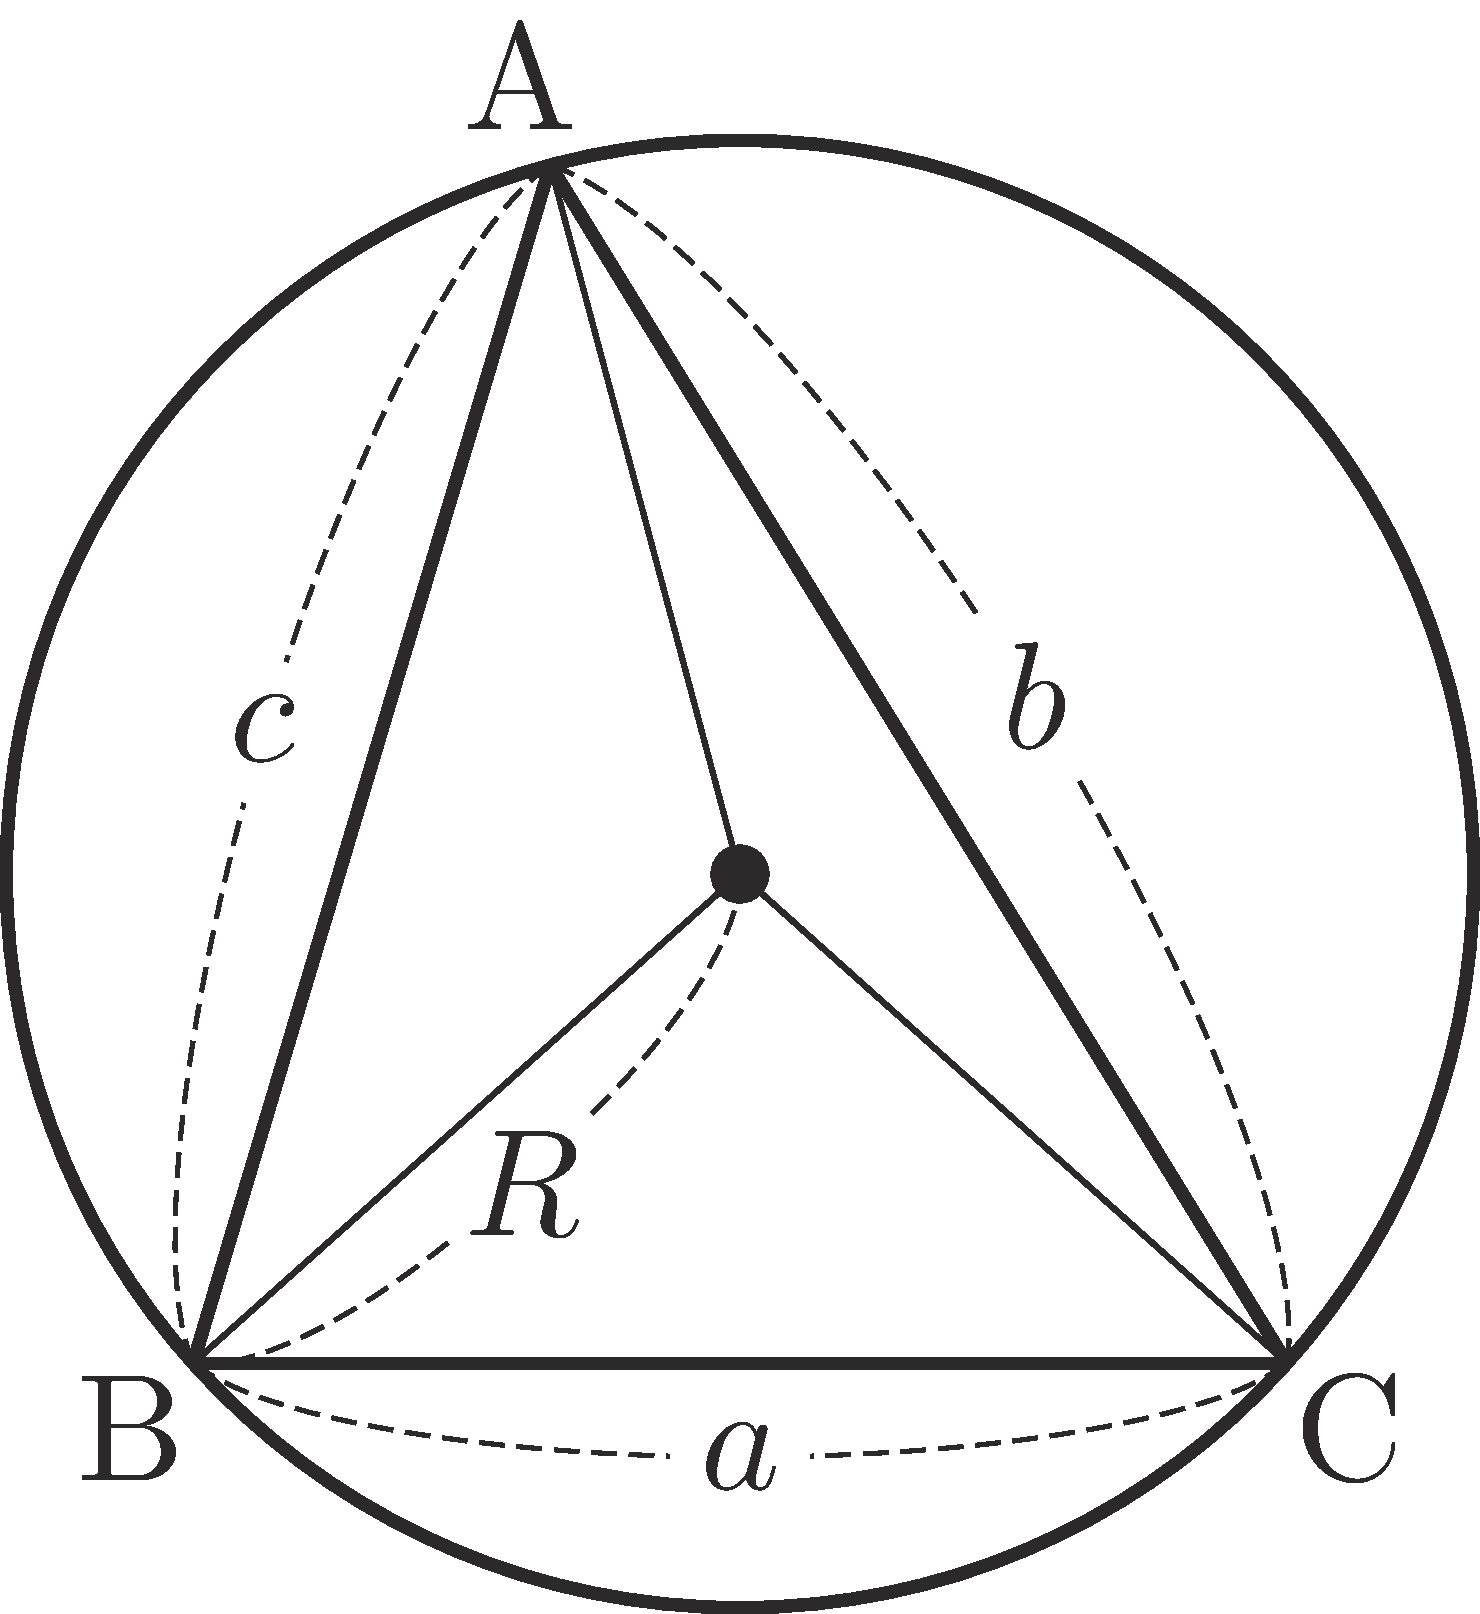
\includegraphics[scale=0.125]{pic0/pic164.pdf}\\
  \end{center}외접원의 반지름의 길이가 $R$인 삼각형 $\mrm{ABC}$에서 $\dfrac{a}{\sin A}=\dfrac{b}{\sin B}=\dfrac{c}{\sin C}=2R$이 성립합니다.\mn{다음과 같은 꼴로 암기하면 세 변의 길이를 즉각 이용할 수 있습니다.\begin{align*}
a &= 2R\sin A \\ 
b &= 2R\sin B \\
c &= 2R\sin C
\end{align*}
}{}
\subsection{코사인법칙}

\begin{figure}[h]
  \centering 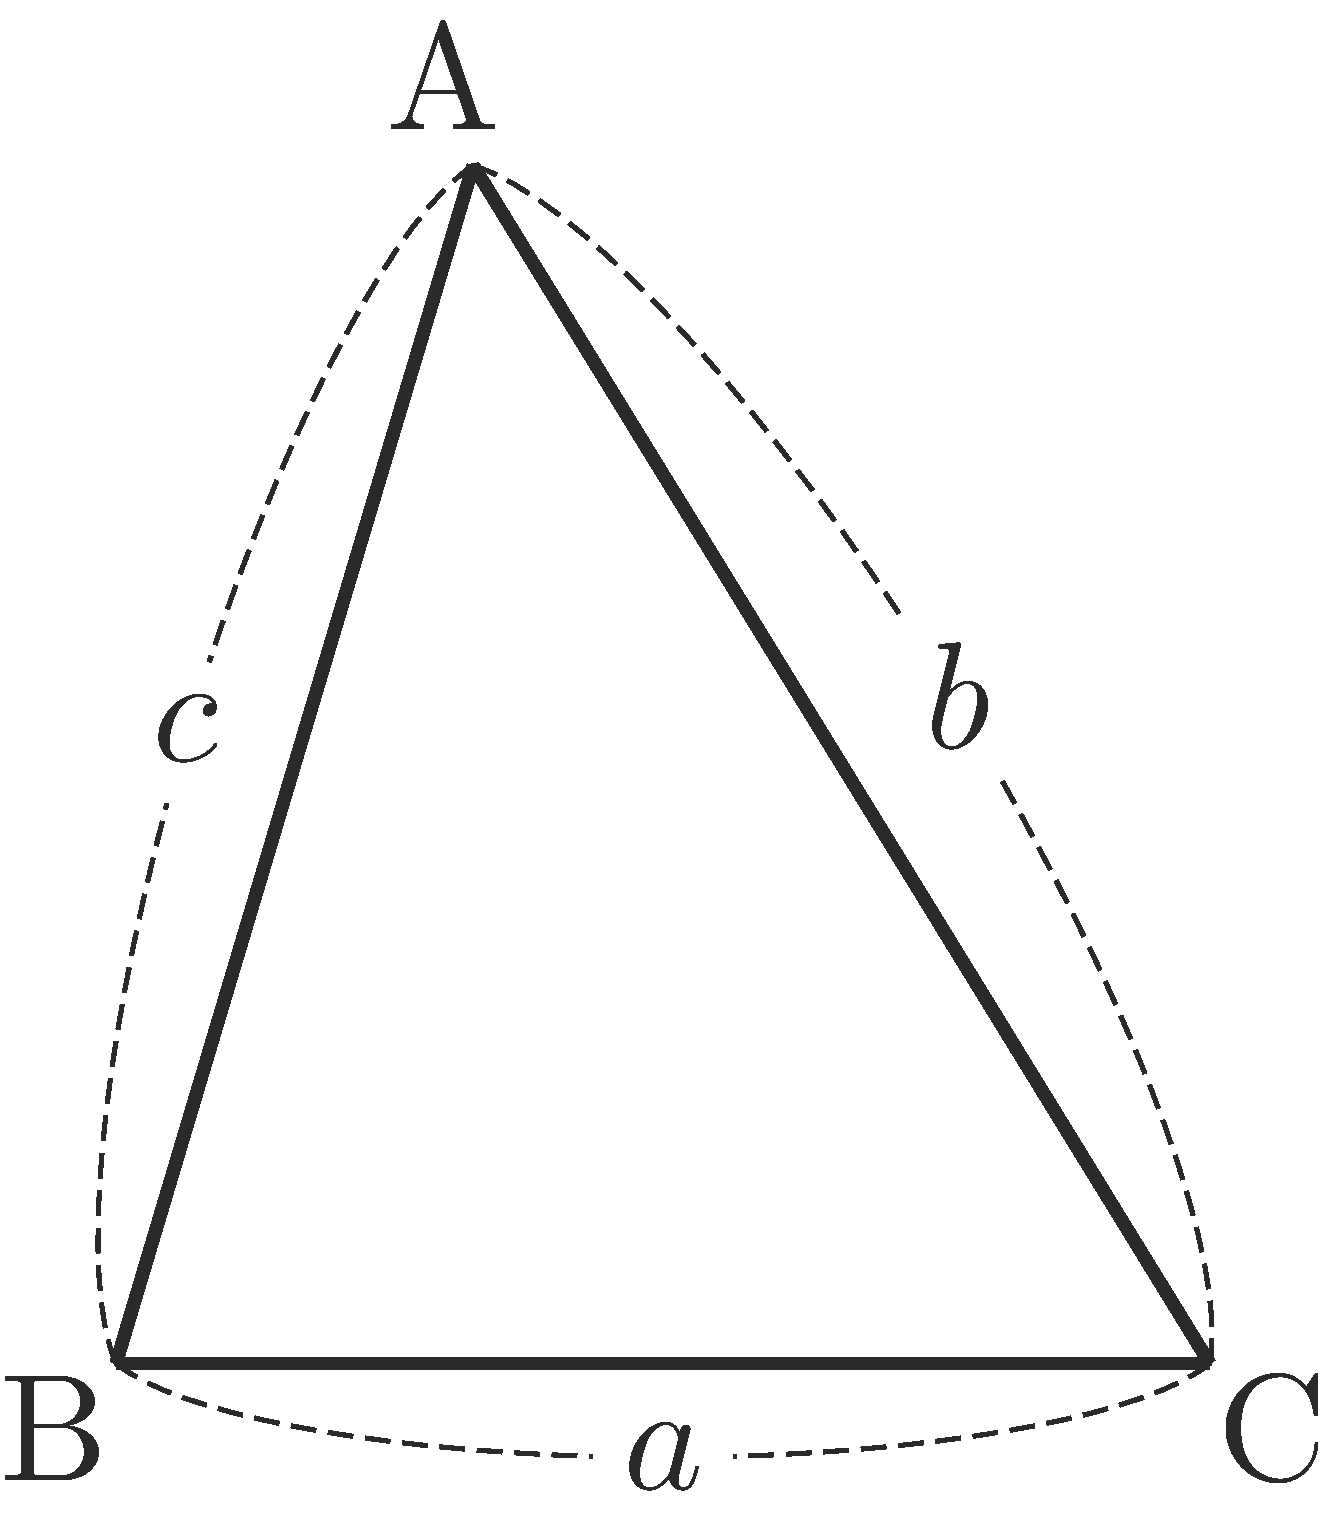
\includegraphics[scale=0.125]{pic0/pic165.pdf}\\
  \end{figure}
삼각형 $\mrm{ABC}$에서 다음이 성립합니다.
\begin{align*}
a^2 &= b^2 + c^2 - 2bc\cos A \\ 
b^2 &= c^2 + a^2 - 2ca\cos B \\
c^2 &= a^2 + b^2 - 2ab\cos C
\end{align*}
\clearpage
\subsection{삼각형의 넓이}\term[넓이!삼각형]{삼각함수를 이용하기}{0}
\begin{center}
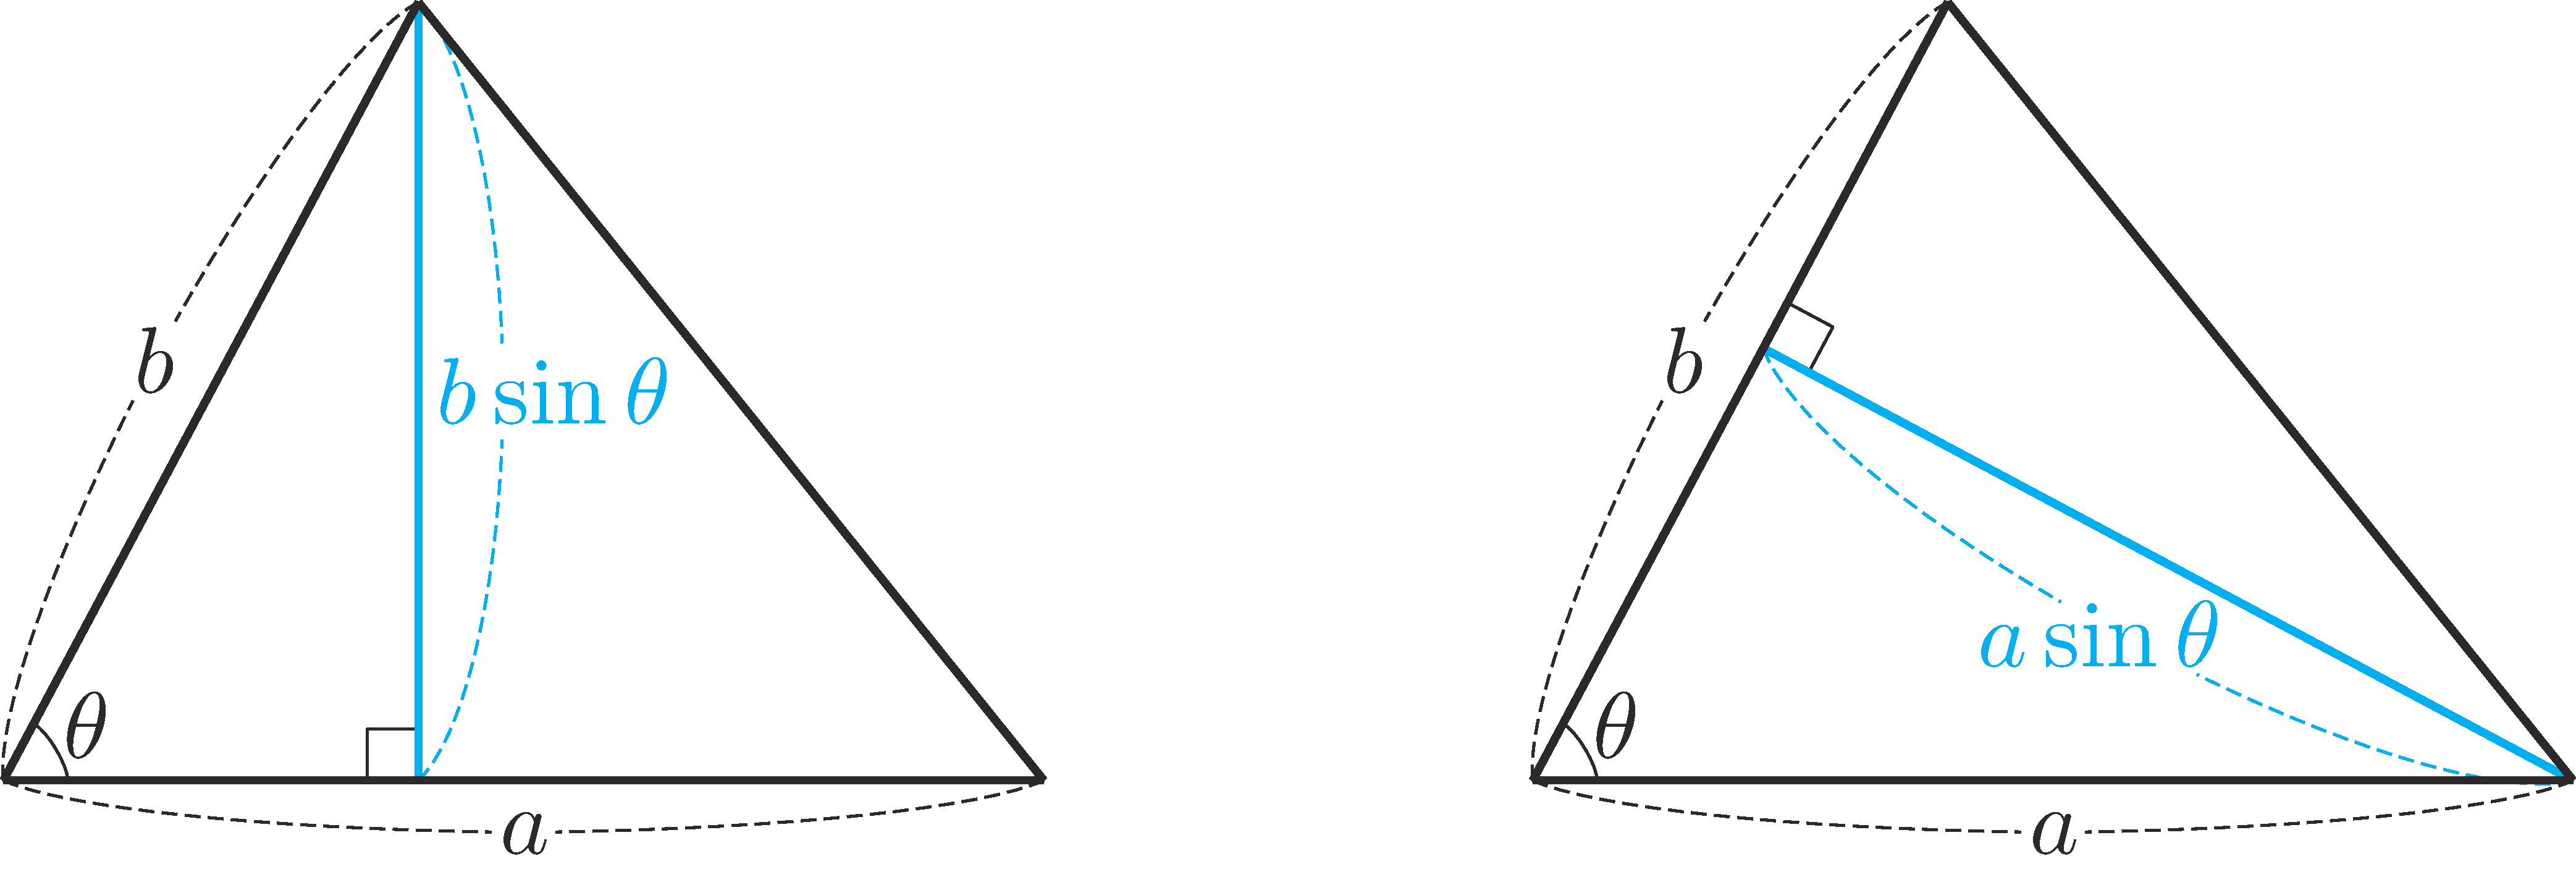
\includegraphics[scale=0.125]{pic0/pic160.pdf}
\end{center}두 변의 길이가 $a$, $b$이고 그 끼인각의 크기가 $\theta$인 삼각형의 넓이는 $\dfrac{1}{2}ab\sin\theta$입니다. 이는 `$a$를 밑변으로 보고 $b\sin\theta$를 높이로 본 것' 또는 `$b$를 밑변으로 보고 $a\sin\theta$를 높이로 본 것'입니다.

\begin{figure}[h]
  \centering 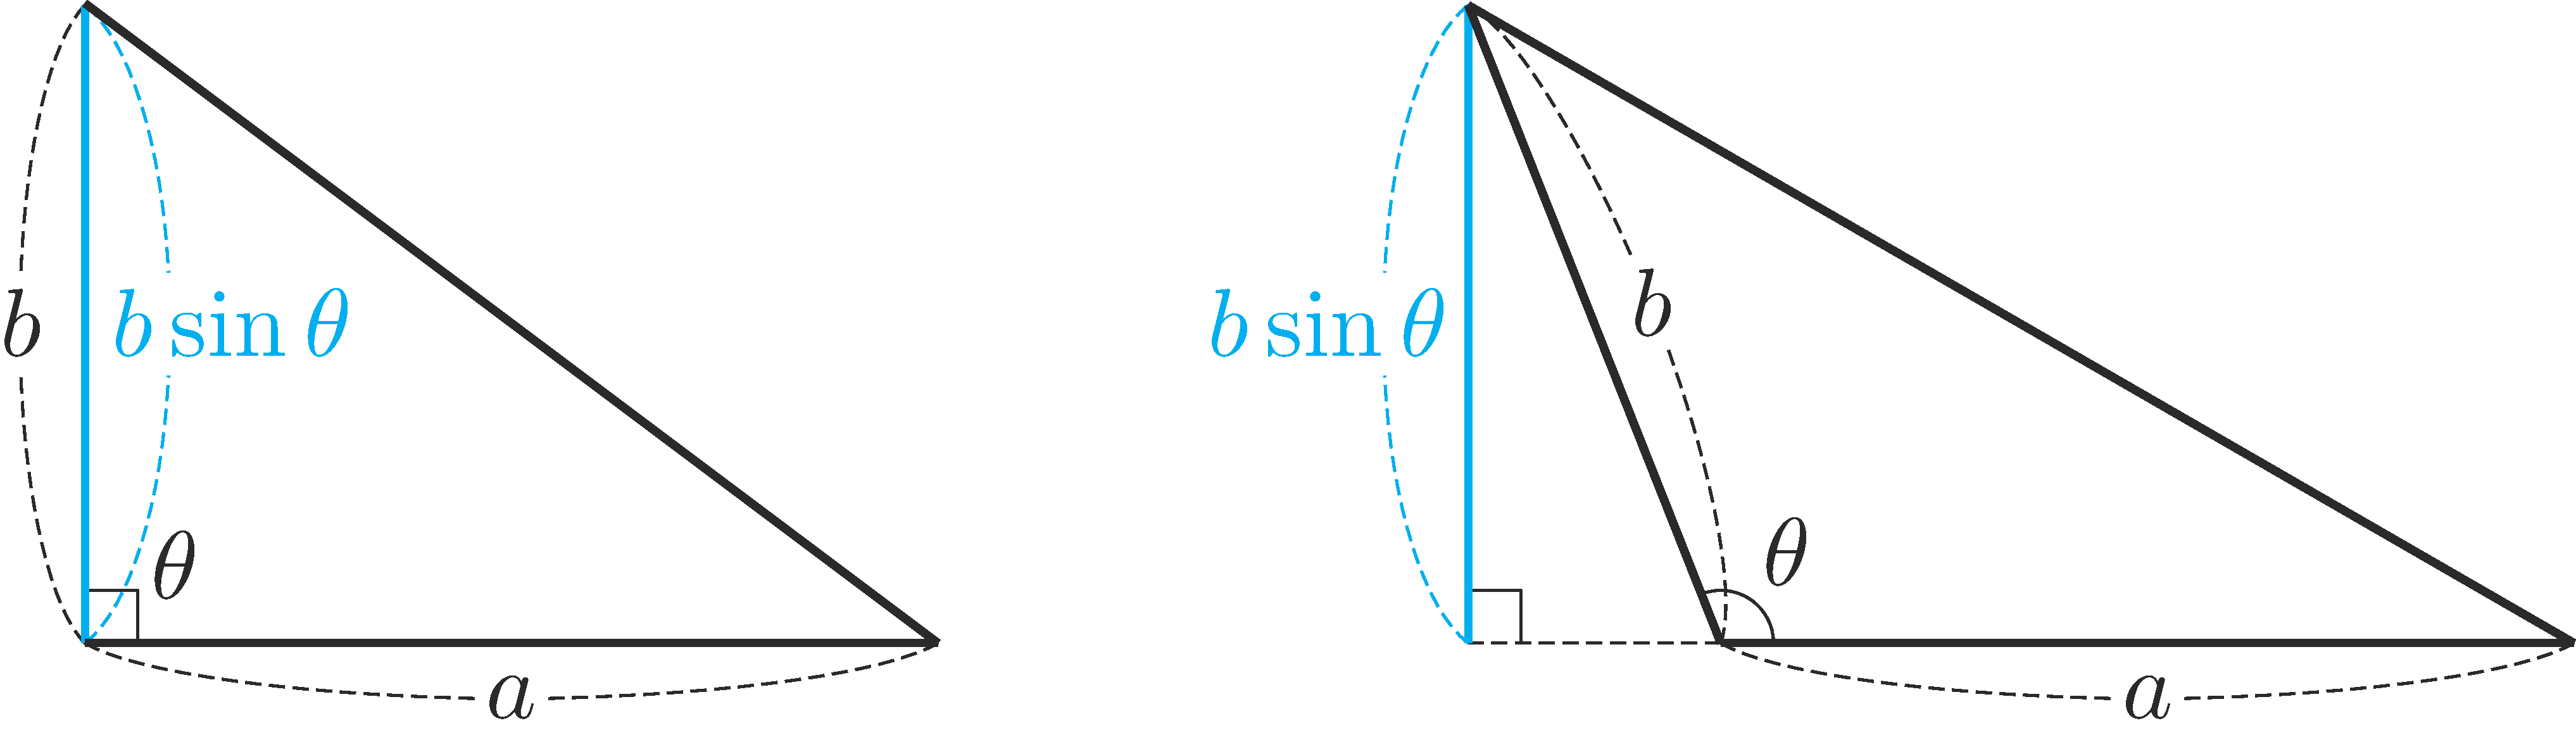
\includegraphics[scale=0.125]{pic0/pic166.pdf}\\
  \end{figure}
이는 $\theta$가 직각이거나 둔각이어도 마찬가지입니다.
